A continuacion, se describe el diseño detallado del sistema Thary, el cual consiste en las siguientes etapas del pipeline:

\subsubsection{Etapa 1: Carga y limpieza de datos}
La primera etapa del pipeline (\texttt{app/services/prediccion/carga\_datos.py}) recibe el archivo CSV cargado por el administrador y lo normaliza hacia un esquema interno unico:


\Needspace{10\baselineskip}
\captionof{listing}{Función \texttt{cargar\_y\_limpiar} y etiquetas de las columnas obligatorias.}\label{lst:carga_limpieza}
\begin{minted}{python}
ETIQUETAS_COLUMNAS_OBLIGATORIAS = {
    "fecha": "Fecha (o Date, Sale_Date)",
    "producto_id": "Código (o Code, Id, Product_ID)",
    "demanda": "Cantidad (o Quantity, Demanda, Demand)",
}

SINONIMOS_COLUMNAS = {
    "fecha": ["Fecha", "Date", "Sale_Date"],
    "producto_id": ["Product_ID", "Codigo", "Code", "Id"],
    "demanda": ["Demanda", "Demand", "Quantity_Sold", "Sales", "Cantidad", "Quantity"],
    # ... variantes adicionales para precio, inventario, categoria, proveedor y lead time
}

NOMBRES_PRODUCTO_AMBIGUOS = ["Producto", "Product"]


def _normalizar_encabezado(nombre):
    """Minúsculas, sin tildes, con espacios/guiones como "_"."""
    texto = unicodedata.normalize("NFKD", str(nombre)).encode("ascii", "ignore").decode()
    return re.sub(r"[\s\-]+", "_", texto.strip().lower())


def _renombrar_columnas(df):
    """Renombra las columnas del archivo a los nombres internos. Si el
    archivo trae "Producto"/"Product" y ademas ya tiene una columna de
    codigo clara (Codigo, Code, Id, Product_ID), esa columna ambigua se
    toma como el NOMBRE del producto en vez de su identificador."""
    # ... logica de resolucion por prioridad y ambiguedad (ver codigo fuente)


def cargar_y_limpiar(ruta_archivo):
    try:
        df = pd.read_csv(ruta_archivo)
    except pd.errors.EmptyDataError:
        raise ValueError("El archivo está vacío. Sube un CSV con al menos una fila de datos.")
    except pd.errors.ParserError:
        raise ValueError(
            "No se pudo leer el archivo como CSV. Verifica que sea un archivo de texto "
            "separado por comas (por ejemplo, no un Excel renombrado a .csv)."
        )
    except UnicodeDecodeError:
        raise ValueError(
            "El archivo tiene una codificación de caracteres que el sistema no reconoce. "
            "Guárdalo como CSV con codificación UTF-8 e intenta de nuevo."
        )

    if df.empty:
        raise ValueError("El archivo no tiene filas de datos, solo encabezados.")

    df = _renombrar_columnas(df)

    columnas_faltantes = [c for c in ETIQUETAS_COLUMNAS_OBLIGATORIAS if c not in df.columns]
    if columnas_faltantes:
        faltan = ", ".join(ETIQUETAS_COLUMNAS_OBLIGATORIAS[c] for c in columnas_faltantes)
        raise ValueError(
            f"Al archivo le falta al menos una columna obligatoria: {faltan}. "
            "Agrégala al CSV (con ese nombre exacto u otro de los aceptados) y vuelve a subirlo."
        )
\end{minted}


En esta sección del archivo (\texttt{app/services/prediccion/carga\_datos.py}), se observa la etapa de carga y limpieza de los datos. Para garantizar que el sistema pueda adaptarse y funcionar para todo tipo de dominio de inventarios, se normalizan los nombres de las columnas de los archivos CSV con el fin de mantener un esquema unico interno, de manera que el sistema pueda aceptar archivos de distintos dominios sin tener la necesidad de modificar el resto del pipeline.

Para facilitarle al usuario el proceso de cargar un archivo, se capturan los errores mas comunes para el sistema a la hora de leer un CSV y se muestran a manera de mensaje de error en un lenguaje sencillo y facil de entender.

Otra practica que fue aplicada es el manejo de errores con mensajes dirigidos al usuario final, de esta manera, se evita que se propaguen los errores internos del sistema y el usuario sabe que es lo que esta ocurriendo y que es lo que se debe hacer para resolverlo.


\subsubsection{Etapa 2: Segmentación de productos}
La segunda etapa del pipeline (\texttt{app/services/prediccion/segmentacion.py}) se basa en poder clasificar cada producto según dos criterios principales:

\begin{itemize}
    \item Clasificación ABC: Esta clasificación permite poder identificar cual es la importancia relativa de cada producto dentro de la demanda total. Se calcula ordenando los productos de mayor a menor en base a su demanda total y se guarda su porcentaje. 
    
    Los productos que en conjunto representan hasta el 80\% de la demanda, se clasifican como categoría A, es decir, los más importantes. Los que se encuentran entre el 80\% y el 95\% se clasifican como categoría B. El resto de productos se clasifican como categoría C.
    
    Esta clasificación permite que en el dashbpard, el usuario pueda entender que tan importante y que tan errático es el consumo de cada producto 
    
    \item Variabilidad: La variabilidad del consumo de los productos permite poder identificar cuales son los productos que presentan un comportamiento más estable y cuales son los que presentan un comportamiento más irregular, se calcula en base al coeficiente de variación (la desviación estándar dividida entre la media de la demanda), clasificando a cada producto como de variabilidad Baja (menor a 0.5), Media (entre 0.5 y 1) o Alta (mayor o igual a 1).

\end{itemize}

\Needspace{10\baselineskip}
\captionof{listing}{Función \texttt{calcular\_comportamiento\_producto}: variabilidad y clasificación ABC de cada producto.}\label{lst:segmentacion}
\begin{minted}{python}
def calcular_comportamiento_producto(df, df_mensual):
    producto_comportamiento = (
        df_mensual.groupby("producto_id")["demanda"]
        .agg(demanda_total="sum", media="mean", desviacion="std")
        .reset_index()
    )
    producto_comportamiento["cv"] = (
        producto_comportamiento["desviacion"] / producto_comportamiento["media"]
    ).replace([np.inf, -np.inf], np.nan)

    def clasificar_variabilidad(cv):
        if pd.isna(cv):
            return "Sin datos"
        if cv < 0.5:
            return "Baja"
        elif cv < 1:
            return "Media"
        else:
            return "Alta"

    producto_comportamiento["variabilidad"] = producto_comportamiento["cv"].apply(clasificar_variabilidad)

    producto_comportamiento = producto_comportamiento.sort_values("demanda_total", ascending=False).reset_index(drop=True)
    total_demanda = producto_comportamiento["demanda_total"].sum()
    if total_demanda > 0:
        producto_comportamiento["demanda_acumulada_pct"] = producto_comportamiento["demanda_total"].cumsum() / total_demanda
    else:
        producto_comportamiento["demanda_acumulada_pct"] = 0

    def clasificar_abc(pct):
        if pct <= 0.80:
            return "A"
        elif pct <= 0.95:
            return "B"
        else:
            return "C"

    producto_comportamiento["categoria_abc"] = producto_comportamiento["demanda_acumulada_pct"].apply(clasificar_abc)

    # ...
    return producto_comportamiento
\end{minted}

Es en esta etapa en la que se calculan estadísticas históricas como (\texttt{media\_producto} y \texttt{desviacion\_producto}).


\subsubsection{Etapa 3: Construcción de variables}
En esta etapa, (\texttt{app/services/prediccion/features.py}), se adapta el historial de demanda a un formato que contenga las variables necesarias que los modelos usan como entrada (\textit{features}):

\begin{itemize}
    \item Componentes de calendario
    \item Rezagos de la demanda
    \item Estadísticas móviles
    \item Estadísticas históricas por producto
\end{itemize}

La implementación de esta etapa empieza con un merge incial, en este merge se trae las categorías abc y variabilidad a la tabla. Aunque no se usan como variables de entrada (\texttt{feature\_cols}), se incluyen porque posteriormente se necesitaran para mostrarlas en el dashboard y tabla de predicciones:

\Needspace{9\baselineskip}
\captionof{listing}{Unión de las categorías ABC y de variabilidad a la tabla mensual.}\label{lst:features_merge}
\begin{minted}{python}
def construir_features(df_mensual, producto_comportamiento):
    # ...
    df_mensual = df_mensual.merge(
        producto_comportamiento[["producto_id", "categoria_abc", "variabilidad"]],
        on="producto_id", how="left"
    )

\end{minted}

Posteriormente, se extraen tanto el año como el mes de cada ejemplo, esto adaptado del repositorio \textit{Demand Forecasting \& Inventory Optimization for Consumer Products} \cite{ejemplo1_demandforecast}, al que en este trabajo se le referira como \textit{Ejemplo 1 (SKU Demand Forecasting)}. Con la diferencia de que en Thary, estos datos se incluyeron con el fin de en la implementación que se tomó como guia, el mes "month", queda como un feature final para el modelo, mientras que en Thary, este dato posteriormente sea tranformado en \texttt{mes\_sin} y \texttt{mes\_cos}, proceso que se explicara más adelante:

\Needspace{4\baselineskip}
\captionof{listing}{Extracción del año y del mes de cada registro.}\label{lst:features_anio_mes}
\begin{minted}{python}
    df_mensual["año"] = df_mensual["fecha"].dt.year
    df_mensual["mes"] = df_mensual["fecha"].dt.month
\end{minted}

Un rezago (lag), se usa en Machine Learning y hace referencia al valor anterior a una variable, en este caso, representa el valor de la demanda del mes anterior, el cual es usado como dato de entrada para predecir el mes actual. Los lags junto con las medias y desviaciones móviles se encargan de capturar el comportamiento reciente de la demanda de cada producto. En Thary, para cada producto se tiene:

\begin{itemize}
    \item lag\_1: demanda del mes anterior
    \item lag\_2: demanda de hace dos meses
    \item lag\_3: demanda de hace tres meses
\end{itemize}

El modelo los usa como features porque la demanda pasada ayuda a poder determinar cuanto se va a vender el proximo mes. Por eso es que un producto necesita mínimo 3 meses de historial antes de los primeros 3 meses del dataset para poder calcular lag1, lag2 y lag3. El problema era que el sistema solo conoce los datos que vienen dentro del mismo archivo CSV que el usuario sube, por lo que no tiene forma de saber que paso antes del primer mes que aparece en el archivo.

Si un dataset empieza en enero de 2021, el lag1 de enero necesitaría la demanda de diciembre de 2020, dato que no esta en el historial dado por el usuario, solo seria a partir de abril 2021 que el sistema contaría con los 3 lags comparados correctamente. Es debido a que no hay información suficiente para calcular los lags correctamente, que el sistema descarta los primeros meses a la hora de entrenar el modelo mediante (\texttt{dropna()}. Como esos primeros 3 meses se descartan,  el valor de mes de esos meses nunca aparece como algo que el modelo tuvo que predecir durante el entrenamiento, por lo que estaría el riesgo de que, si más adelante se le pide al modelo predecir justo ese mismo mes del año siguiente (por ejemplo, enero 2022), el modelo no tenga ninguna referencia previa de que número de mes es ese, y termine adivinando mal, generando predicciones muy bajas o poco confiables para ese mes en particular

Para evitar este problema, se decidió que durante esta etapa de features, se representaría el mes utilizando seno y coseno en vez de usar directamente el número del mes (1-12). Esto permite que el modelo interprete el mes como un punto continuo cercano a los meses vecinos que si fueron entrenados, por ejemplo, diciembre y enero quedan numericamente uno cerca del otro, lo cual tiene mucho más sentido que hacer que el sistema los vea como el número 12 y 1, valores mucho más lejanos de lo que deberían ser para dos meses vecinos. 

Una vez que el modelo entienda la cercania real de los meses, es capaz de dejar de interpretarlos como categorías independientes, y puede generar una predicción razonable de un mes que nunca halla visto antes (enero, por ejemlo), en base la información de un mes cercano (diciembre).

A la hora de armar la función para construir los features se tomaron en cuenta diferentes implementaciones previas de distintos estudios con diferentes propuestas para un sistema de predicción de demanda, se compararon y se seleccionaron aquellas que se apataban mejor a las necesidades del sistema y le aportaban valos al mismo, junto con la implementación de nuevas ideas y mejoras que se fueron propuestas e implemantadas en Thary. Una de estas propuestas nuevas fue la codificación ciclica del mes, que como ya se explicó antes, consiste en representar los meses mediante dos valores calculados con seno y coseno, como se puede ver a continuación:

\Needspace{5\baselineskip}
\captionof{listing}{Codificación cíclica del mes mediante seno y coseno.}\label{lst:features_ciclico}
\begin{minted}{python}
    # ...
    df_mensual["mes_sin"] = np.sin(2 * np.pi * df_mensual["mes"] / 12)
    df_mensual["mes_cos"] = np.cos(2 * np.pi * df_mensual["mes"] / 12)
\end{minted}

Por otra parte, la metodologia de implementar el uso de lags, también se tomó del \textit{Ejemplo 1 (SKU Demand Forecasting)} \cite{ejemplo1_demandforecast} y se adaptó a las necesidades del sistema Thary, agregando la codificación cíclica de los meses y la inclusión de features adicionales como el inventario y el precio.

\Needspace{8\baselineskip}
\captionof{listing}{Cálculo de los rezagos \texttt{lag\_1}, \texttt{lag\_2}, \texttt{lag\_3} y \texttt{lag\_6} por producto.}\label{lst:features_lags}
\begin{minted}{python}
    # ... 
    # (Ejemplo 1 - SKU Demand Forecasting)
    df_mensual["lag_1"] = df_mensual.groupby("producto_id")["demanda"].shift(1)
    df_mensual["lag_2"] = df_mensual.groupby("producto_id")["demanda"].shift(2)
    df_mensual["lag_3"] = df_mensual.groupby("producto_id")["demanda"].shift(3)
    df_mensual["lag_6"] = df_mensual.groupby("producto_id")["demanda"].shift(6)
\end{minted}

Otra estrategia que se tomó del \textit{Ejemplo 1 (SKU Demand Forecasting)} \cite{ejemplo1_demandforecast}, fue el uso de las estadísticas móviles. Estas aportan al sistema ya que consisten en un resumen de varios meses juntos. Mientras que los rezagos solo representan cuanto se vendió exactamente en un mes, las estadísticas móviles son un resumen de varios meses juntos.

\begin{itemize}
\item \texttt{media\_movil\_3} y \texttt{media\_movil\_6}: Estas variables representan cual es el nivel reciente de la demanda de los productos calculando el promedio de los últimos 3 y 6 meses. Esto ayuda que el modelo pueda distingir un producto que vende de manera estable de uno irregular, ya que de ser ventas regulares, la media móvil de 3 meses será muy similar a la de 6 meses, mientras que si es inestable, ambas medias serán muy diferentes.
\item \texttt{desviacion\_movil\_3}: Representa que tan errática fue la demanda reciente, es decir, de los últimos 3 meses. Los productos que cuentan con demanda estable tendrán una desviación baja mientras que los productos con ventas inestable tendrán una desviación alta.
\end{itemize}

En general, el modelo puede ver el comportamiento general reciente de los productos más allá de solo los lags.

En cuanto a la implementación, se incluyó en la función de (\texttt{construir\_features}), en el que cada línea calcula por producto (\texttt{groupby("producto\_id")}) una estadística sobre una ventana de meses anteriores (\texttt{.shift(1)}) para no incluir el mes actual, evitando fuga de datos.


\Needspace{10\baselineskip}
\captionof{listing}{Cálculo de las estadísticas móviles \texttt{media\_movil\_3}, \texttt{media\_movil\_6} y \texttt{desviacion\_movil\_3}.}\label{lst:features_moviles}
\begin{minted}{python}
    # ...
    # (Ejemplo 1 - SKU Demand Forecasting)

    df_mensual["media_movil_3"] = df_mensual.groupby("producto_id")["demanda"].transform(
        lambda x: x.shift(1).rolling(3).mean()
    )
    df_mensual["media_movil_6"] = df_mensual.groupby("producto_id")["demanda"].transform(
        lambda x: x.shift(1).rolling(6).mean()
    )
    df_mensual["desviacion_movil_3"] = df_mensual.groupby("producto_id")["demanda"].transform(
        lambda x: x.shift(1).rolling(3).std()
    )
\end{minted}

Por otra parte, para la construcción de la etapa de Features también se tomó en cuenta el repositorio en Kaggle \textit{Forecasting Inventory Demand Using XGBoost} \cite{ejemplo3_ksmooi_inventorydemand} o \textit{Ejemplo 3 (XGBoost)} \cite{ejemplo3_ksmooi_inventorydemand}. De este repositorio, se tomó el uso de el promedio del producto, pero esta vez, calculados en base a todo el historial completo y no solo en base a los últimos 3 o 6 meses. 

Como extensión propuesta por el proyecto, junto al promedio también se incluyó la desviación del producto, esto para poder seguir una misma estructura en todo el sistema, ya que si se tiene la (\texttt{media\_movil\_3}) y la (\texttt{desviacion\_movil\_3}), es decir, el nivel y la variabilidad de los últimos 3 meses, es conveniente tener la media y desviación de todo el historial del producto.

Estos valores ya fueron calculados en la etapa de segmentación, y simplemente son agregados en los features para que el modelo también los use como variables de entrada.

\Needspace{10\baselineskip}
\captionof{listing}{Incorporación de la media y la desviación históricas de cada producto.}\label{lst:features_historicas}
\begin{minted}{python}
    # ...
    # (Forecasting Inventory Demand Using XGBoost)
    stats_cols = ["demanda_total", "media", "desviacion"]
    df_mensual = df_mensual.merge(
        producto_comportamiento[["producto_id"] + stats_cols].rename(
            columns={"media": "media_producto", "desviacion": "desviacion_producto"}
        ),
        on="producto_id", how="left"
    )
\end{minted}

Después, se calculca cuanto stock habia el mes anterior. La condición (\texttt{if "inventario" in df\_mensual.columns:}) determina si el csv que fue subido por el usuario contiene la columna "inventario", esta es una columna opcional que simplemente representa cuantas unidades de ese producto (stock disponible) habia fisicamente en el inventario en ese mes, Thary funciona sin ella, pero si el usuario la incluye, el modelo la usara como una variable de entrada más para poder brindarle un análisis mucho más detallado. 

(\texttt{(inventario\_lag\_1)}) es el inventario del mes anterior, con (\texttt{.groupby("producto\_id")}) se asegura que este se calcule por separado para cada producto, esto con la intención de evitar que el inventario de un producto se vaya a mezclar con otro, esto usando (\texttt{(shift(1))}) para poder obtener el inventario del mes anterior. Si no se hace esto, el modelo podría aprender que el inventario de un producto es igual al del mes actual, lo cual no es correcto y generaría predicciones erroneas. 

\Needspace{6\baselineskip}
\captionof{listing}{Cálculo del inventario del mes anterior (\texttt{inventario\_lag\_1}).}\label{lst:features_inventario_lag}
\begin{minted}{python}
    # ...
    # (Forecasting Inventory Demand Using XGBoost))
    if "inventario" in df_mensual.columns:
        df_mensual["inventario_lag_1"] = df_mensual.groupby("producto_id")["inventario"].shift(1)
\end{minted}

En esta parte, se implementó otra idea del \textit{Ejemplo 1 (SKU Demand Forecasting)} \cite{ejemplo1_demandforecast} para poder descartar las filas sin historial suficiente para tener los lags. Para esto, se define una lista con nueve nombres de las columnas obligatorias para poder entrenar, con (\texttt{(dropna(subset=feature\_history))}) se revisan las 4 columnas y elimina cualquier fila que tenga un espacio vacío, posteriormente el resultado se guarda en (\texttt{(df\_model)}), que es la tabla final que se usara para entrenar el modelo.

\Needspace{10\baselineskip}
\captionof{listing}{Descarte de las filas sin historial suficiente para calcular los rezagos.}\label{lst:features_dropna}
\begin{minted}{python}
    # ...
    # (Inventory Demand Forecast (XGBoost Reg))
    feature_history = ["lag_1", "lag_2", "lag_3", "media_movil_3"]
    df_model = df_mensual.dropna(subset=feature_history).copy()

    if len(df_model) == 0:
        raise ValueError(
            "Ningún producto tiene al menos 3 meses seguidos de historial, que es lo mínimo "
            "para calcular tendencias. Sube un archivo con más meses continuos de datos."
        )
\end{minted}

Otro de los conceptos que fueron propuestos en Thary es el tratamiento que se decidió darle a la variable con los precios de venta de los productos. Aunque el CSV pueda incluir esa variable, el modelo solo usa su valor actual (el precio de ese mes), sin calcular cómo cambió respecto al mes anterior. Esto debido a que por naturaleza, el precio de un producto puede influir en la demanda de un producto, ya que cuando algo baja de precio, la gente tiende a comprar más, mientras que cuando este sube, las personas compran menos. El problema es que si esta regla se repite muy seguido, se corre el riesgo de que el modelo aprenda que el cambio de precio predice muy bien la demanda, entonces, aunque el precio es una variable que si se tiene en cuenta, se excluye por completo su variabilidad de un mes a otro.  

\Needspace{10\baselineskip}
\captionof{listing}{Lista de variables de entrada (\texttt{feature\_cols}) y variables opcionales de precio e inventario.}\label{lst:features_lista}
\begin{minted}{python}
    # ...
    feature_cols = [
        "año", "mes_sin", "mes_cos",
        "lag_1", "lag_2", "lag_3", "lag_6",
        "media_movil_3", "media_movil_6", "desviacion_movil_3",
        "media_producto", "desviacion_producto"
    ]
    if "precio" in df_model.columns:
        feature_cols.append("precio")
    if "inventario" in df_model.columns:
        feature_cols.append("inventario")
        if "inventario_lag_1" in df_model.columns:
            feature_cols.append("inventario_lag_1")
\end{minted}

Finalmente, como extensión propia de Thary, se hace un relleno final. Para esto, se recorre cada una de las columnas que van a usar los modelos, si hay alguna fila vavia en la tabla, se reemplazan los vacios de la columna con 0 mediante (\texttt{df\_model[col] = df\_model[col].fillna(0)}). Esto es importante porque si el modelo recibe un producto que solo aparece a partir de cierto mes, por ejemplo, abril 2021 en un dataset que empieza en enero de ese mismo año, el mes de abril pudo pasar el filtro de dropna() porque ya tiene (\texttt{(lag\_1, lag\_2, lag\_3 y media\_movil\_3 completos)}, pero en este caso, el lag\_6 necesitaría la demanda de octubre de 2020, mes que no existe en el archivo porque el producto todavua no tiene 6 meses de historial.

La fila pasaría el filtro porque \texttt{lag\_6} no está en \texttt{feature\_history}, pero inevitablemente terminará en \texttt{feature\_cols}, y ahí es donde se ejecuta este bloque final, si \texttt{lag\_6} es vacío en esa fila se rellena con 0.

\Needspace{6\baselineskip}
\captionof{listing}{Relleno final de los valores vacíos de las variables de entrada con 0.}\label{lst:features_relleno}
\begin{minted}{python}
    # ...
    for col in feature_cols:
        if df_model[col].isna().any():
            df_model[col] = df_model[col].fillna(0)
\end{minted}


\subsubsection{Etapa 4: Modelos de predicción}
Esta etapa se reparte en los siguientes archivos:

\begin{itemize}
\item \texttt{app/services/prediccion/modelos.py}
\item \texttt{app/services/prediccion/regresion\_lineal.py}
\end{itemize}

\paragraph{Definición de variables y funciones basicas}

Al incio del archivo \texttt{modelos.py}, se define el nivel de significancia \texttt{NIVEL\_SIGNIFICANCIA\_DM} como 5\%, esta variable se va a usar posteriormente a la hora de evaluar si un resultado es estadísticamente significativo:

\Needspace{3\baselineskip}
\captionof{listing}{Nivel de significancia de la prueba de Diebold-Mariano.}\label{lst:nivel_significancia}
\begin{minted}{python}
NIVEL_SIGNIFICANCIA_DM = 0.05
\end{minted}

Como parte de la propuesta de Thary,también se implemenaron las siguientes cuatro variables:

\Needspace{7\baselineskip}
\captionof{listing}{Constantes que definen el tamaño del periodo de prueba (\textit{backtest}).}\label{lst:constantes_backtest}
\begin{minted}{python}
MESES_ARCHIVO_UMBRAL_TEST_GRANDE = 18
TEST_SIZE_MESES_DEFAULT = 3
TEST_SIZE_MESES_GRANDE = 6

MESES_PERDIDOS_POR_REZAGOS = 3
\end{minted}

Por defecto, el periodo de prueba son 3 meses, pero cuando se cuenta con un periodo de prueba más grande, de 18 meses o más, este pasa de 3 meses a 6 meses.

Esta decisión se tomó después de identificar un problema con el que contaba el sistema. Como punto de partida, el sistema elige el mejor modelo para cada producto comparando el MAE de los 3 modelos sobre 3 meses del historial, el problema era que con solo 3 meses, el resultado podría no ser lo suficientemente confiable, esto debido a que con tan pocos datos, un solo mes que sea atípico puede terminar haciendo que un modelo "gane" sin que eso refleje una diferencia real, sobretodo porque el MAE es una medición que cuenta con mucha varianza. Entre los riesgos identificados se encuentra: poca capacidad de distinguir modelos parecidos, inestabilidad del resultado y sesgo estacional.

Antes de llegar a la solución definitva se planteo una primera propuesta, en la que si el archivo contaba con menos de 18 meses, se haría la comparación del MAE de los 3 modelos sobre 3 meses, pero si contaba con 18 meses o más, la comparación se haría sobre 6 meses. Pero enrealidad, esta solución no resolvia el problema "de raiz", solo mitigaba el problema de que hubiera pocos meses de prueba, además de que la decisión de que 18 meses fuese el punto de corte no tenia respaldo alguno.

Por eso fue que se corrigió y re-interpretó el enfoque de la solución, fundamentándola en que el problema a solucionar no era el número de meses, sino el cálculo del error, es decir, qué tan confiable es la comparación de error entre los modelos.

Fue aquí donde se propuso la prueba Diebold-Mariano, la cual consiste en una prueba estadística que permite medir si la diferencia de error que hay entre dos modelos es significativa o es solo ruido. La prueba Diebold-Mariano requiere de un nivel de significancia, que se definió como 5\%.

Por otro lado,\texttt{MESES\_PERDIDOS\_POR\_REZAGOS} es el número fijo de meses que se pierden al calcular los rezagos (visto en la etapa anterior), es necesario para disctribuir los meses utilizables del total de meses que subió el usuario en el archivo.

Una vez definidas las variables, la primera función implementada en \texttt{modelos.py} es \texttt{tamano\_test\_backtest}. Esta función principalmente se encarga de implementar la solución ya explicada, recibe como parámetro \texttt{n\_meses\_usables}, la cantidad de meses que quedaron disponibles después de que se hayan perdido los primeros por el cálculo de los lags, y devuelve cuántos meses de esos son los que se van a usar como período de prueba (backtest).

\Needspace{7\baselineskip}
\captionof{listing}{Función \texttt{tamano\_test\_backtest}, que decide el tamaño del periodo de prueba.}\label{lst:tamano_test_modelos}
\begin{minted}{python}
def tamano_test_backtest(n_meses_usables):
    n_meses_archivo_original = n_meses_usables + MESES_PERDIDOS_POR_REZAGOS
    if n_meses_archivo_original >= MESES_ARCHIVO_UMBRAL_TEST_GRANDE:
        return TEST_SIZE_MESES_GRANDE
    return TEST_SIZE_MESES_DEFAULT
\end{minted}

Como el umbral de decisión (\texttt{MESES\_ARCHIVO\_UMBRAL\_TEST\_GRANDE = 18}) toma en cuenta el archivo completo, y la función recibe la cantidad de meses disponibles ya con los 3 meses de lag descontados, con \texttt{n\_meses\_archivo\_original = n\_meses\_usables + MESES\_PERDIDOS\_POR\_REZAGOS} se le suma esos 3 meses de vuelta, para saber cuántos meses tenía el archivo que el usuario subió originalmente

Luego se compara si el total de meses completo cuenta con 18 meses, de hacelo devuelvve el tamaño de test grande con 6 meses y de no hacerlo devuelve el tamaño de test por defecto de 3 meses.

Esta función se llama desde \texttt{sistema\_prediccion.py}, para decidir el tamaño del split que se usa para elegir el campeón y generar los resultados, y desde \texttt{validacion.py}, para que los \textit{folds} de la validación cruzada temporal usen ese mismo tamaño de test y conservar un criterio estandarizado en ambas partes.

Es parte de la solución que se propone en Thary, esta función no ninguna en alguna de las implementaciones que fueron revisadas ya que ninguna adapta el tamaño del perido de prueba seun la cantidad de historia disponible. 

\paragraph{Modelos de demanda}

Las funciones que permiten entrenar y evaluar los tres modelos de demanda que se van a utilizar en el sistema: Media Móvil, Regresión Lineal y XGBoost. Estos fueron elegidos luego de realizar una revisión de literatura en la que se compararon 5 modelos para la predicción de la demanda, tal como se vio en el capítulo "Antecedentes", de los cuales se escogieron: XgBoost y regresión lineal al ser los que presentan mejor desempeño en este tipo de problemas, y adicionalmente se incluyó media móvil como un modelo más sencillo que puede ser útil para productos con demanda estable o que no cuenten con suficiente historial implementar para un modelo más complejo.

\paragraph{Implementación de XgBoost}

La implementación de XGBoost se hizo combinando los hiperparametros de \textit{Ejemplo 1 (SKU Demand Forecasting)} \cite{ejemplo1_demandforecast} con la transformación del objetivo propuesta en \textit{Ejemplo 3 (XGBoost)} \cite{ejemplo3_ksmooi_inventorydemand}.


\textit{Ejemplo 3 (XGBoost)} \cite{ejemplo3_ksmooi_inventorydemand} cuenta con una configuración muchísimo mas simple de la que necesitaría Thary, ya que en el caso del ejemplo, se estaba trabajando con aproximadamente 60 millones de filas, por lo que se priorizó la velocidad sobre el ajuste fino de hiperparámetros, por lo que no cuenta con factores como algún control de sobreajuste:


\Needspace{8\baselineskip}
\captionof{listing}{Parámetros del modelo XGBoost del \textit{Ejemplo 3}.}\label{lst:xgboost_ejemplo3}
\begin{minted}{python}
# Define the parameters for the XGBoost model
params = {
    'max_depth': 8,                  # Maximum depth of a tree
    'eta': 0.5,                      # Learning rate
    'objective': 'reg:squarederror'  # Objective function for regression
}
\end{minted}


Por otra parte, el \textit{Ejemplo 1 (SKU Demand Forecasting)} \cite{ejemplo1_demandforecast} si cuenta con una configuración mas completa que se podría reutilizar, en este se arma un XGBRegressor mas cuidado en el que se incluyen variables como \texttt{n\_estimators=300}, \texttt{learning\_rate=0.05}, \texttt{subsample=0.8}, \texttt{colsample\_bytree=0.8}, pero principalmente se escogió seguir la lógica de este ejemplo porque de los cuatro ejemplos revisados, es el único que consiste en un sistema completo con una premisa bastante similar a la de Thary, ya que ofrece pronóstico de demanda, traducción de ese pronóstico en recomendaciones de reposición, punto de reorden, EOQ, y todo eso bajo restricciones de lead time y presupuesto.

Es por eso, que se adoptó su enfoque general completo:

\begin{itemize}
    \item Variables
    \item modelos
    \item hiperparametros
    \item comparación de modelos
    \item lógica de reposición
\end{itemize}

Los otros ejemplos se revisaron posteriormente cuando se necesitó mejorar aspectos, agregar nuevas funcionalidades o en general, agregarle mas valor y robustez a Thary.

Los hiperparámetros utilizados parten de los mismos que se encuentran en el \textit{Ejemplo 1 (SKU Demand Forecasting)} \cite{ejemplo1_demandforecast}. Como ya se explicó anteriormente, al ser el ejemplo más cercano a una implementación completa de un sistema con las características de Thary, se optó por mantener su lógica de entrenamiento y ajuste de hiperparámetros , con la diferencia de que \texttt{n\_estimators} se aumentó de 300 a 500, y \texttt{objective} se fijó explícitamente en \texttt{reg:squarederror}, mientras que en el ejemplo original no se especificaba. Esto se cambió ya que se buscaba implementar el uso de mínimos cuadrados para poder estimar la bondad de los modelos.

Parámetros como \texttt{verbosity} fueron omitidos en Thary, pero se incluyó \texttt{n\_jobs}, el cual permite utilizar todos los núcleos de procesamiento disponibles en la máquina donde se ejecuta el entrenamiento, en lugar de un único núcleo. Esto contribuye a reducir el tiempo de entrenamiento del modelo cuando se procesan catálogos con un número elevado de productos.

\Needspace{10\baselineskip}
\captionof{listing}{Función \texttt{entrenar\_xgboost}, con los hiperparámetros del modelo.}\label{lst:entrenar_xgboost}
\begin{minted}{python}
def entrenar_xgboost(X_train, y_train_log, X_test):
    model = xgb.XGBRegressor(
        objective="reg:squarederror", n_estimators=500, 
        learning_rate=0.05,
        max_depth=4, 
        subsample=0.8, 
        colsample_bytree=0.8,
        reg_alpha=0.1, 
        reg_lambda=1.0, 
        random_state=42, 
        n_jobs=-1
    )
    model.fit(X_train, y_train_log)
    pred_xgb = model.predict(X_test)
    pred_xgb = np.maximum(np.expm1(pred_xgb), 0)
    return model, pred_xgb
\end{minted}

Cada uno de estos hiperparámetros tiene un impacto específico en cómo se entrena el modelo, y a continuación se explica qué efecto tiene el valor elegido para Thary:

\begin{itemize}
    \item \texttt{n\_estimators=500}: Es la cantidad de árboles que se entrenan uno tras otro. Con más árboles, el modelo tiene más oportunidades de corregir los errores que va dejando cada árbol anterior, pero también tarda más en entrenarse. El Ejemplo 1 usa \texttt{n\_estimators=300}; se subió a 500 porque, al combinarse con una tasa de aprendizaje baja (\texttt{learning\_rate=0.05}), se necesitan más árboles para que el modelo aprenda lo suficiente. Para confirmar que este cambio ayudaba, se probó con distintas cantidades de árboles (de 100 a 1200): con 300 (el valor original del Ejemplo 1) el error fue mayor que con 500, y subir más allá de 500 lo seguía bajando, pero muy poco (menos de 1\% entre 500 y 1200), mientras que el tiempo de entrenamiento se triplicaba. Se eligió 500 por ser una mejora real sobre el valor original, sin pagar un tiempo de entrenamiento mucho mayor para una ganancia casi nula, algo relevante porque el modelo se vuelve a entrenar cada vez que un usuario sube un archivo.

    \item \texttt{learning\_rate=0.05}: Es la tasa de aprendizaje (\textit{shrinkage}), y controla cuánto peso se le da a cada árbol nuevo que se agrega (Sección 2.2.9). Con un valor bajo como 0.05, cada árbol individual aporta poco al resultado final, por lo que se necesitan muchos árboles (de ahí los 500) para que el modelo aprenda bien, pero a cambio, el modelo es menos propenso a memorizar el ruido de los datos de entrenamiento. Este valor es idéntico al del Ejemplo 1.

    \item \texttt{max\_depth=4}: Limita cuántas divisiones puede hacer cada árbol (Sección 2.2.9). Con una profundidad de 4, cada árbol es relativamente simple, lo que evita que un solo árbol se vuelva demasiado complejo y termine memorizando patrones muy específicos de los datos de entrenamiento en vez de aprender el comportamiento general de la demanda. Este valor es idéntico al del Ejemplo 1.

    \item \texttt{subsample=0.8}: En cada árbol nuevo, solo se usa el 80\% de las filas de entrenamiento, escogidas al azar (Sección 2.2.9). Esto hace que los árboles no vean siempre exactamente los mismos datos, lo que ayuda a que el modelo generalice mejor en vez de ajustarse demasiado a casos particulares del historial. Este valor es idéntico al del Ejemplo 1.

    \item \texttt{colsample\_bytree=0.8}: De manera similar al anterior, pero con las variables (columnas): cada árbol solo usa el 80\% de las variables disponibles, también escogidas al azar. Esto evita que el modelo dependa siempre de las mismas variables para todos los árboles, lo que también ayuda a que generalice mejor. Este valor es idéntico al del Ejemplo 1.

    \item \texttt{reg\_alpha=0.1} y \texttt{reg\_lambda=1.0}: Son los términos de regularización L1 y L2 que penalizan la complejidad de cada árbol (Sección 2.2.9). Un valor más alto hace que el modelo sea más conservador, prefiriendo árboles más simples. Los dos valores se mantuvieron idénticos al Ejemplo 1. Al probar otros valores de \texttt{reg\_alpha} sobre el archivo del caso de estudio, el resultado con 0.1 fue muy parecido al de no usar esta regularización, así que se conservó el valor del Ejemplo 1 sin necesidad de cambiarlo.

    \item \texttt{random\_state=42}: No afecta el resultado del modelo en sí, sino que fija la semilla aleatoria que se usa en el \texttt{subsample} y el \texttt{colsample\_bytree}, para que cada vez que se entrene el modelo con los mismos datos, se obtenga exactamente el mismo resultado. Este valor también es idéntico al del Ejemplo 1.

    \item \texttt{n\_jobs=-1}: Le indica a XGBoost que use todos los núcleos de procesamiento disponibles en la máquina, en vez de uno solo, lo que reduce el tiempo de entrenamiento cuando se procesan catálogos con muchos productos. Este parámetro no viene del Ejemplo 1 (que no lo específica); se agregó en Thary porque no afecta el resultado del modelo, solo la velocidad de entrenamiento.
\end{itemize}

En cuanto a la transformación logarítmica, se implementó siguiendo la lógica del \textit{Ejemplo 3 (XGBoost)} \cite{ejemplo3_ksmooi_inventorydemand}, en el que el modelo no entrena directamente sobre \texttt{y\_train}, que sería la demanda real, sino sobre \texttt{y\_train\_log}, que es la transformación logarítmica de \texttt{y\_train}.


Esto porque en la vida real, la demanda suele tener una distribución en la que puede haber muchos productos con demanda baja y pocos con picos muy altos. Si se entrenara directamente sobre esos valores el modelo podría enfocarse demasiado en los pocos casos extremos, esto llevaría a que se prediciera peor la mayoría de los casos normales. El logaritmo lo que hace es parejar esa diferencia: hace que los valores muy grandes dejen de pesar tanto en comparación con los valores más pequeños, así el modelo le presta atención equilibrada a todos los productos y no solo a los que tienen demanda extrema. Se usa \texttt{log1p} porque la demanda puede valer 0, y el logaritmo de 0 no existe.



\paragraph{Implementación de Media Móvil}

Media móvil hace referencia al método más simple de los tres. La técnica con la que se implementó también se basa fuertemente en el \textit{Ejemplo 1 (SKU Demand Forecasting)} \cite{ejemplo1_demandforecast}, y consiste en simplemente reutilizar la columna de \texttt{media\_movil\_3} que ya se tiene desde la etapa anterior de features. No se tiene que hacer ningún entrenamiento.

\Needspace{4\baselineskip}
\captionof{listing}{Función \texttt{prediccion\_baseline\_movil}, que implementa el modelo de media móvil.}\label{lst:prediccion_media_movil}
\begin{minted}{python}
def prediccion_baseline_movil(test_df):
    return np.maximum(test_df["media_movil_3"].values, 0)
\end{minted}

La función recibe como parámetro el \texttt{test\_df} y posteriormente, para todas las filas, devuelve el valor \texttt{media\_movil\_3} que ya se había calculado anteriormente.

El único parámetro relevante de este modelo es el tamaño de la ventana que se promedia, en este caso, 3 meses (\texttt{media\_movil\_3}). Una ventana más pequeña haría que el modelo reaccionara más rápido a cambios recientes en la demanda, pero también lo haría más sensible a meses atípicos. Una ventana más grande suavizaría más el resultado, pero tardaría más en reflejar cambios reales en el comportamiento de un producto. Se eligió 3 meses siguiendo la misma lógica del Ejemplo 1 (SKU Demand Forecasting) \cite{ejemplo1_demandforecast}, que también usa una ventana de este tamaño.

\paragraph{Implementación de Regresión Lineal}

Para implementar regresión lineal, se adaptó la lógica del \textit{Ejemplo 4 (BoomBikes)} \cite{ejemplo4_boombikes}, al ser el modelo que más pasos requiere, se implementó de manera individual en el archivo \texttt{regresion\_lineal.py}.

\Needspace{6\baselineskip}
\captionof{listing}{Filtro de las columnas sin variación (función \texttt{\_seleccionar\_features\_regresion}).}\label{lst:regresion_candidatas}
\begin{minted}{python}
    def _seleccionar_features_regresion(X_train, y_train, max_p_valor=0.05, max_vif=5.0):
        candidatas = [c for c in X_train.columns if X_train[c].std() > 0]
        if len(candidatas) < 2 or len(X_train) <= len(candidatas) + 1:
            return candidatas
\end{minted}

Inicialmente, se filtran y excluyen las columnas que no varian demasiado, descartando las que tienen una desviación estándar de 0, ya que una desviación estándar con este valor indica que en esas columnas el valor es siempre el mismo número.

con \texttt{std() > 0}, esto se hace porque cuando se entrena regresión lineal, no siempre conviene usar todas las variables disponibles porque no todas tienen algo significativo que aportar. Es incluso perjudicial para el modelo, ya que una columna sin variación no le sirve de nada al modelo (no hay nada que "aprender" de un número que nunca cambia).

Posteriormente, se convierten todos los valores de cada columna a un rango entre 0 y 1, para mantener las proporciones relativas con \texttt{MinMaxScaler}. Se ajusta \texttt{fit\_transform} usando solo los datos con los que se hace el entrenamiento, no se puede incluir a los de prueba porque eso haría que el sistema vea los datos que se supone debe predecir.  

\Needspace{8\baselineskip}
\captionof{listing}{Escalado de las variables con \texttt{MinMaxScaler}.}\label{lst:regresion_escalado}
\begin{minted}{python}
    try:
        scaler = MinMaxScaler()
        X_train_esc = pd.DataFrame(
            scaler.fit_transform(X_train[candidatas]),
            columns=candidatas, index=X_train.index
        )
\end{minted}

En esta parte se incluye Recursive Feature Elimination (RFE). Este consiste en un método que entrena varias veces un modelo de regresión lineal, y en cada una se elimina la variable que aporte menos al modelo hasta que al final, se quede con un número controlado de variables, en este caso, tienen que ser 2 variables como mínimo para posteriormente poder realizar el análisis, pero no pueden ser más de 8 variables porque no se pueden dejar demasiadas \texttt{n\_rfe = max(2, min(8, len(candidatas) - 1))}.

El \texttt{n\_rfe} define cuantas variables como máximo puede conservar el proceso de RFE (entre 2 y 8, según \texttt{n\_rfe = max(2, min(8, len(candidatas) - 1))}). El límite inferior de 2 garantiza que quede al menos una variable además de la más importante, y el límite superior de 8 evita que el modelo termine con demasiadas variables, ya que aunque RFE ya descarta las menos importantes, un número muy alto de variables restantes haría más lento el resto del proceso de selección (VIF y p-valor), que se aplican después sobre las que sobrevivan a RFE.

Finalmente, \texttt{seleccionadas} es la lista de columnas que sobrevivieron esta primera etapa, aunque es posible que aún existan variables redundantes:

\Needspace{6\baselineskip}
\captionof{listing}{Selección de variables mediante \textit{Recursive Feature Elimination} (RFE).}\label{lst:regresion_rfe}
\begin{minted}{python}
    n_rfe = max(2, min(8, len(candidatas) - 1))
    rfe = RFE(LinearRegression(), n_features_to_select=n_rfe)
    rfe.fit(X_train_esc, y_train)
    seleccionadas = [c for c, usar in zip(candidatas, rfe.support_) if usar]
\end{minted}

La segunda etapa para seleccionar varibles consiste en calcular el VIF o Factor de Inflación de Varianza para cada variable. Este se encarga de medir que tan redundante es una variable en comparación con las demas, el criterio para decidir esto es estimar si una variable se puede predecir con exactitud a partir de las otras, de ser este el caso, su VIF será muy alto y eso es un problema porque el modelo no podría distinguir cuál de las dos variables redundantes es la que esta causando el efecto.

En la implementación de Thary, entre las variables que se considerian redundantes se encuentran:

\begin{itemize}
    \item \texttt{inventario} y \texttt{inventario\_lag\_1}: Escencialmente tienden a ser casi la misma variable, en muchos casos, es bastante probable que el inventario de un mes sea bastante parecido al del mes anterior.
    \item Los lags (\texttt{lag\_1}, \texttt{lag\_2}, \texttt{lag\_3}, \texttt{lag\_6}): También es comun que la demanda de un producto tienda a ser similar a la de meses anteriores, si un producto vendió bien un mes, es muy probable que también venda mes el siguiente mes, lo que a la larga hace que los lags sean variables muy parecidas entre si.
    \item (\texttt{media\_movil\_3} y \texttt{media\_movil\_6}) con los lags: Que todos los Lags sean similares llevaría a que, inevitablemente, la media móvil de 3 meses y la de 6 meses también lo sean debido a que se calculan a partir de promediar los lags.
    \item (\texttt{media\_producto}) y las medias móviles: (\texttt{media\_producto}) consiste en el promedio histórico general del producto, si los productos cuentan con un comportamiento estable, es probable que sea similar a (\texttt{media\_movil\_3} y \texttt{media\_movil\_6}), por lo que también se considera una variable redundante.
\end{itemize}

Teniendo esto en cuenta, las variables que no se considerarian redundantes son: \texttt{año}, \texttt{mes\_cos}, \texttt{mes\_sin}, \texttt{desviacion\_movil\_3} y \texttt{desviacion\_producto}.

\Needspace{10\baselineskip}
\captionof{listing}{Cálculo del VIF de las variables seleccionadas.}\label{lst:regresion_vif}
\begin{minted}{python}
    while len(seleccionadas) > 1:
        X_sm = sm.add_constant(X_train_esc[seleccionadas])
        with warnings.catch_warnings():
            warnings.simplefilter("ignore", category=SingularMatrixWarning)
            warnings.simplefilter("ignore", category=UserWarning)
            vif = pd.DataFrame({
                "feature": seleccionadas,
                "VIF": [variance_inflation_factor(X_sm.values, i + 1) for i in range(len(seleccionadas))]
            })
\end{minted}

Posteriormente, se quitan las variables con un VIF infinito que nisiquiera se puede calcular, ya que de ser este el caso, significaria que la variable es tan redundante con otra que rompe las matemáticas del modelo. Esto ocurriria porque a la hora de calcular los coeficientes de la regresión lineal, el algoritmo necesita calcular cuanto aporta cada variable a la predicción, y para eso, necesita poder distinguir el efecto individual de cada una. El problema es que si dos variables son casi idénticas entre sí , es imposible distinguirlas.

Es por eso, que en esta etapa esas variables son eliminadas.En las siguientes líneas de código, se revisa cual variable tiene el VIF más alto si ya no hay variables con VIF infinito, si el valor del vif más alto supera el límite que se definió en \texttt{max\_vif}, esa variable se elimina y finalmente se vuelve a repetir el proceso desde el principio hasta que se halla calculado el VIF de las variables restantes y todas estas cuenten con un VIF menor al límite establecido.

\Needspace{10\baselineskip}
\captionof{listing}{Eliminación de variables con VIF infinito o superior al límite.}\label{lst:regresion_eliminacion_vif}
\begin{minted}{python}
    vif_problema = vif[~np.isfinite(vif["VIF"])]
    if not vif_problema.empty:
        seleccionadas.remove(vif_problema.iloc[0]["feature"])
        continue

    peor_vif_fila = vif.loc[vif["VIF"].idxmax()]
    if peor_vif_fila["VIF"] > max_vif:
        seleccionadas.remove(peor_vif_fila["feature"])
        continue
\end{minted}

Una vez completado el proceso de eliminación de las variables redundantes, se prosigue con la implementación del entrenamiento del modelo de regresión lineal, en el que se revisa el "p-valor" de cada variable. 

El P-valor consiste en una medida estadística que indica que tan probable es que la variable que se esta revisando este relacionada con la demanda solo por casualidad y no porque de verdad dicha variable este relacionada de verdad con la demanda. En este caso, si se encuentra que la variable que cuenta con el peor p-valor supera el límite de \texttt{max\_p\_valor}, que es estandarizado como 0.05 al representar el 95\% de confianza en estadística, se elimina la variable y se repite el proceso. 

El bucle se detiene cuando ya no haya ninguna variable con el VIF alto o con el P-valor alto, al cumplir con ambos criterios, solo se contara con variables limpias y estadísticamente significativas para el proceso. 

De haber algún fallo durante esta etapa, simplemente se devuelve la lista completa de variables con el fin de garantizar de que el pipeline no se rompa y el sistema pueda continuar funcionando.

\Needspace{10\baselineskip}
\captionof{listing}{Eliminación de variables según el p-valor del modelo OLS.}\label{lst:regresion_pvalor}
\begin{minted}{python}
        modelo_ols = sm.OLS(y_train, X_sm).fit()
        p_valores = modelo_ols.pvalues.drop("const")
        peor_p_nombre = p_valores.idxmax()
        peor_p_valor = p_valores[peor_p_nombre]

        if peor_p_valor > max_p_valor:
            seleccionadas.remove(peor_p_nombre)
        else:
            break

    return seleccionadas
except Exception:
    return candidatas
\end{minted}

Por otro lado, en ese mismo archivo, se implementó la función \texttt{entrenar\_regresion\_lineal}, que se encarga de entrenar el modelo de regresión lineal y devolver las predicciones, también es a la que se llama desde el resto del sistema.

La función llama a \texttt{\_seleccionar\_features\_regresion} para obtener la lista de variables que se van a usar en el entrenamiento del modelo, (si por algún motivo, dicha función le devuelve una lista que se encuentre vacia, se usan todas las variables originales.)

El modelo es entrenado con las variables limpias asegurandose que las predicciones no sean negativas al no ser algo que tenga sentido en este contexto. 

Finalmente, devuelve el modelo entrenado, las predicciones y la lista de variables que se usaron para entrenar el modelo.

\Needspace{10\baselineskip}
\captionof{listing}{Función \texttt{entrenar\_regresion\_lineal}, que entrena el modelo con las variables seleccionadas.}\label{lst:entrenar_regresion_lineal}
\begin{minted}{python}
def entrenar_regresion_lineal(X_train, y_train, X_test, feature_cols):
    features_lr = _seleccionar_features_regresion(X_train, y_train)
    if not features_lr:
        features_lr = list(feature_cols)

    modelo_lr = LinearRegression()
    modelo_lr.fit(X_train[features_lr], y_train)
    pred_lr = modelo_lr.predict(X_test[features_lr])
    pred_lr = np.maximum(pred_lr, 0)

    return modelo_lr, pred_lr, features_lr

\end{minted}


\subsubsection{Selección del campeón por producto}
El sistema de prediccion Thary no usa el mismo metodo para todos los productos del catalogo. Para cada uno de los productos se selecciona cual de los tres modelos candidatos usar para su pronostico. 

Esta desicion se tomo de manera independiente para el sistema Thary, ya que al revisar las implementaciones de los 4 sistemas de prediccion en las que se baso el sistema, se evidencio que estos simplemente usaban el mejor modelo para todo el catalogo por igual.

En una primera version del sistema, la seleccion del mejor modelo por producto se hacia en base a cual de los 3 obtuvo un menor MAE. El problema con esta estrategia es que el backtest generalmente solo cuenta con entre 3 y 6 meses de datos si es que se cuenta con un archivo mas grande, son pocos meses, por lo que el hecho de que un modelo tenga el MAE mas bajo no es prueba de que sea mejor, podria darse por diferentes factores o por casualidad. 

Es por eso que para seleccionar el mejor modelo, lo primero que se hace es calcular el MAE de los 3 modelos, se identifican los dos modelos que obtengan el menor MAE para cada producto. Esto usando \texttt{np.argsort} sobre la tabla de errores:

\Needspace{10\baselineskip}
\captionof{listing}{Identificación del mejor y el segundo mejor modelo de cada producto (función \texttt{elegir\_campeon\_por\_producto}).}\label{lst:campeon_mejores}
\begin{minted}{python}
def elegir_campeon_por_producto(resultados_prediccion):
    errores_por_metodo = pd.DataFrame({
        metodo: (resultados_prediccion["demanda"] - resultados_prediccion[columna]).abs()
        for metodo, columna in COLUMNA_PREDICCION_POR_METODO.items()
    })
    productos = resultados_prediccion["producto_id"]
    errores_por_producto = errores_por_metodo.groupby(productos).mean()

    metodos = errores_por_producto.columns.to_numpy()
    orden = np.argsort(errores_por_producto.to_numpy(), axis=1)
    mejor_metodo = pd.Series(metodos[orden[:, 0]], index=errores_por_producto.index)
    segundo_metodo = pd.Series(metodos[orden[:, 1]], index=errores_por_producto.index)
\end{minted}

Se calcula la diferencia de error entre el mejor y el segundo mejor modelo para cada uno de los productos mes a mes, y se resume esa diferencia con su media, desviación estándar y cantidad de observaciones:

\Needspace{10\baselineskip}
\captionof{listing}{Diferencia de error entre el mejor y el segundo mejor modelo.}\label{lst:campeon_diferencias}
\begin{minted}{python}
    mejor_por_fila = productos.map(mejor_metodo)
    segundo_por_fila = productos.map(segundo_metodo)
    error_mejor = np.select(
        [mejor_por_fila == metodo for metodo in errores_por_metodo.columns],
        [errores_por_metodo[metodo] for metodo in errores_por_metodo.columns],
    )
    error_segundo = np.select(
        [segundo_por_fila == metodo for metodo in errores_por_metodo.columns],
        [errores_por_metodo[metodo] for metodo in errores_por_metodo.columns],
    )
    diferencia = pd.Series(error_mejor - error_segundo, index=resultados_prediccion.index)
    stats_diferencia = diferencia.groupby(productos).agg(d_media="mean", d_std="std", n="count")
\end{minted}

Se implemento la prueba de Diebold-Mariano \cite{diebold_mariano}. El problema que resuelve es que cuando se comparan dos modelos para un producto, se quiere saber si el modelo ganador realmente es mejor o si por algun motivo tuvo suerte en esos pocos 3 meses, ya que un solo mes con un comportamiento atipico puede hacer que un modelo gane sin que eso signifique que sea mejor.

La prueba Diebold-Mariano permite determinar estadisticamente si la diferencia de error entre el mejor y el segundo mejor modelo es estadisticamente significativa, o si es solo ruido. La prueba consiste en observar mes a mes cuanto le gano un modelo al otro. Si esa diferencia es consistente (un modelo le gana al otro casi todos los meses, por una cantidad parecida), es una señal fuerte de que la ventaja es real. Si la diferencia varia mucho de un mes a otro (a veces gana uno, a veces el otro, por cantidades muy distintas), es señal de que lo que se vio como "ganador" fue mas bien casualidad.

Debido a que la prueba clasica esta pensada para muestras grandes, se adapto para muestras pequeñas siguiendo la correccion de Harvey, Leybourne y Newbold, ampliamente discutida y recomendada por Diebold \cite{diebold2015comparing}, la cual consistio en ajustar (\texttt{dm\_ajustado = dm * sqrt((n-1)/n)}) y comparar el resultado contra una distribucion t de Student con n-1 grados de libertad, en vez de la normal estandar de la prueba original. Cuantos mas grados de libertad tiene una prueba estadistica, mas confiable es su capacidad de detectar diferencias reales, especialmente cuando se cuenta con pocos datos.

La implementacion de la prueba consiste, inicialmente, en medir que tan confiable es el promedio de las diferencias, dado que se calculo con pocos datos. Cuanto mas dispersas son las diferencias (\texttt{d\_std}) o menos meses tiene (\texttt{n}), mas "ruidoso" es ese promedio.

Para comparar que tan grande es la ventaja promedio frente a que tan confiable es: si la ventaja promedio es grande pero el error estandar (la inconsistencia) tambien es grande, \texttt{dm} resulta pequeño, lo cual es señal de que la ventaja no es confiable.

\Needspace{10\baselineskip}
\captionof{listing}{Prueba de Diebold-Mariano con la corrección de Harvey, Leybourne y Newbold.}\label{lst:campeon_diebold_mariano}
\begin{minted}{python}
        error_estandar = stats_diferencia["d_std"] / np.sqrt(stats_diferencia["n"])
        dm = stats_diferencia["d_media"] / error_estandar
        correccion_hln = np.sqrt((stats_diferencia["n"] - 1) / stats_diferencia["n"])
        dm_ajustado = dm * correccion_hln
        grados_libertad = (stats_diferencia["n"] - 1).clip(lower=1)
        p_valor = pd.Series(
            2 * (1 - stats.t.cdf(dm_ajustado.abs(), df=grados_libertad)),
            index=stats_diferencia.index,
        )

    suficientes_datos = stats_diferencia["n"] >= 2
    sin_varianza = stats_diferencia["d_std"].fillna(0) == 0
    significativo = suficientes_datos & (p_valor < NIVEL_SIGNIFICANCIA_DM) & ~sin_varianza

    campeon = mejor_metodo.copy()
    campeon[~significativo] = "Media móvil"
    return campeon
\end{minted}

Se descarta el resultado del MAE y se usa el modelo de Media Movil como respaldo si:

\begin{itemize}
    \item La diferencia no resulta estadisticamente significativa, es decir, que el p-valor de la prueba Diebold-Mariano es mayor al nivel de significancia definido (5\%).
    \item Los dos métodos se equivocaron exactamente igual (varianza cero, sin evidencia de que uno sea mejor)
    \item No hay al menos 2 meses para medir varianza
\end{itemize}

En estos casos se selecciona la Media Movil en vez del modelo que gano por una diferencia que no es significativa y que podria tratarse solo de ruido.

Al aplicar este mecanismo al sistema, se evidencio un cambio drastico en el resultado real, probado sobre el catalogo completo de la Clinica Nuestra Señora de los Remedios (856 productos). Antes de implementar la validacion con Diebold-Mariano, seleccionando unicamente por el MAE mas bajo, el metodo campeon se distribuia asi:

\begin{itemize}
    \item XGBoost ganaba en 430 productos (50.2\%)
    \item Media Movil en 227 (26.5\%)
    \item Regresion Lineal en 199 (23.2\%)
\end{itemize}

Al incorporar la prueba de Diebold-Mariano, esa distribucion cambio radicalmente: 

\begin{itemize}
    \item XGBoost paso a ganar en solo 15 productos (1.8\%)
    \item Regresion Lineal en 12 (1.4\%)
    \item Media Movil paso a ser el metodo campeon en 829 productos (96.8\%)
\end{itemize}


De los 430 productos en los que originalmente ganaba XGBoost, 415 pasaron a usar Media Movil y solo 15 se mantuvieron con XGBoost; de los 199 en los que ganaba Regresion Lineal, 187 pasaron a Media Movil y solo 12 se mantuvieron. Los 227 productos que ya usaban Media Movil se mantuvieron igual, ya que este es el metodo de respaldo cuando la diferencia no resulta significativa. 

Esto evidencia que, sin la validacion estadistica de Diebold-Mariano, el sistema estaba seleccionando modelos "ganadores" cuya ventaja, en la gran mayoria de los casos, no era estadisticamente distinguible del ruido.

En cuanto al tamaño del periodo de prueba, cuando se cuenta con un test fijo de 3 meses, la prueba de Diebold-Mariano siempre tendria solo 2 grados de libertad, sin importar cuanta historia tenga el archivo, nunca ganando mas poder estadistico para detectar diferencias reales. Por eso, el tamaño del periodo de prueba se ajusta segun el historial disponible:

\Needspace{7\baselineskip}
\captionof{listing}{Función \texttt{tamano\_test\_backtest}, que ajusta el periodo de prueba al historial disponible.}\label{lst:campeon_tamano_test}
\begin{minted}{python}
def tamano_test_backtest(n_meses_usables):
    n_meses_archivo_original = n_meses_usables + MESES_PERDIDOS_POR_REZAGOS
    if n_meses_archivo_original >= MESES_ARCHIVO_UMBRAL_TEST_GRANDE:
        return TEST_SIZE_MESES_GRANDE
    return TEST_SIZE_MESES_DEFAULT
\end{minted}

En caso de que se cuente con un archivo csv grande (es decir, un archivo con 18 meses o mas), se usa un test de 6 meses en vez de 3, dandole mas grados de libertad y mas poder estadistico a la prueba de Diebold-Mariano. 

El corte de 18 meses es practica definida para este proyecto, se escogio por ser un valor redondo (año y medio). No es un valor tomado de una fuente externa, a diferencia del las demas practicas aplicadas como Diebold-Mariano o nivel de significancia.

\subsubsection{Combinación de pronósticos (análisis complementario)}
Además de seleccionar un modelo por producto, se quiso evaluar si combinar dos modelos aporta algún valor en comparación con usar uno solo. Este análisis se agregó de manera independiente para el sistema Thary, ya que ninguna de las 4 implementaciones de referencia combina modelos. La idea viene de la literatura de combinación de pronósticos \cite{bates1969combination, granger1984improved}, que se explica en la Sección 2.1.

Un aspecto importante es que esta combinación no participa en la predicción que usa Thary en producción ni en la selección del modelo campeón, sino que solo se muestra en el panel técnico del administrador como un análisis complementario.

Se combinan las predicciones de XGBoost y Media Móvil porque, de los tres modelos candidatos, son los que obtuvieron mejores resultados en la validación (Tabla \ref{tab:resumen_cv}). Lo primero es calcular el peso $w$ que se le da a XGBoost, ya que a la Media Móvil le corresponde $1 - w$. Esto se hace con la fórmula de mínimos cuadrados explicada en la Sección 2.1, en la función \texttt{\_peso\_minimos\_cuadrados}:

\Needspace{10\baselineskip}
\captionof{listing}{Cálculo del peso de la combinación (función \texttt{\_peso\_minimos\_cuadrados}).}\label{lst:combinacion_peso}
\begin{minted}{python}
def _peso_minimos_cuadrados(y, pred_a, pred_b):
    diferencia = pred_a - pred_b
    denominador = float(np.sum(diferencia ** 2))
    if denominador == 0:
        return 0.5
    w = float(np.sum((y - pred_b) * diferencia) / denominador)
    return min(max(w, 0.0), 1.0)
\end{minted}

Aquí \texttt{y} es la demanda real, \texttt{pred\_a} es la predicción de XGBoost y \texttt{pred\_b} la de Media Móvil, y el cálculo del peso es la misma fórmula presentada en la Sección 2.1, aplicada sobre todas las filas del backtest. Hay dos casos especiales. El primero es que si las dos predicciones son idénticas, el denominador es cero, y como no hay nada que decidir entre un modelo y otro, el peso es 0.5, lo que además evita dividir entre cero. El segundo es que el resultado se recorta entre 0 y 1 con \texttt{min} y \texttt{max}, para que la combinación siempre sea un promedio ponderado, ya que si la demanda real queda fuera del rango entre las dos predicciones, la fórmula daría un peso mayor a 1 o menor a 0.

Para saber si la combinación realmente mejora los resultados, se compara contra XGBoost solo y Media Móvil sola sobre las mismas filas del backtest. Un aspecto importante es que el peso de cada mes se calcula sin usar ese mes, sino solo con los demás meses del backtest:

\Needspace{10\baselineskip}
\captionof{listing}{Cálculo del peso de cada mes sin usar ese mes (función \texttt{evaluar\_combinacion}).}\label{lst:combinacion_evaluacion}
\begin{minted}{python}
for mes in np.unique(meses):
    es_mes = meses == mes
    resto = ~es_mes
    if resto.any():
        w = _peso_minimos_cuadrados(y[resto], pred_xgb[resto], pred_mm[resto])
    else:
        w = 0.5

    pesos_por_mes[str(mes)] = round(w, 4)
    combinada[es_mes] = w * pred_xgb[es_mes] + (1 - w) * pred_mm[es_mes]
\end{minted}

Esto se hace porque si el peso se calculara con los mismos datos contra los que después se mide el error, el peso ya habría "visto" las respuestas de antemano y la combinación saldría artificialmente buena, que es el mismo principio de no hacer trampa que se explicó en la validación del modelo. Además, como los productos se juntan en un solo cálculo, hay miles de filas para calcular cada peso aunque cada producto tenga pocos meses. Si solo existe un mes, no quedan datos para calcular el peso y se usa 0.5.

Como resultado, la función devuelve las métricas (MAE, RMSE, Mediana del Error, R\textsuperscript{2}, MAPE y WAPE) de las tres opciones: Media Móvil sola, XGBoost solo y la combinación. También devuelve el peso final calculado con todos los meses, y cuánto mejora la combinación respecto al mejor de los dos modelos solos, en porcentaje de MAE y de RMSE. Un valor positivo significa que la combinación es mejor, y uno negativo que es peor. Esta función cuenta con 7 pruebas automatizadas, descritas en la Sección 3.4.1.

\subsubsection{Pronóstico futuro}
El cálculo del pronóstico futuro es la funcionalidad principal del sistema, es decir, predecir la demanda de los productos en los meses posteriores al último mes del archivo CSV cargado por el usuario.

Después de que el usuario sube el archivo CSV con el historial de consumo, el sistema le permite configurar tanto el presupuesto disponible como el número de meses que desea pronosticar. Se implementó en \texttt{app/services/prediccion/pronostico\_futuro.py}:

\Needspace{18\baselineskip}
\captionof{listing}{Función \texttt{generar\_pronostico\_futuro}, que arma la lista de meses a pronosticar.}\label{lst:generar_pronostico_futuro}
\begin{minted}{python}
def generar_pronostico_futuro(
    df_mensual, producto_comportamiento, model, feature_cols, modelo_lr, features_lr,
    horizonte_meses=HORIZONTE_MESES_DEFAULT,
):
    proximo_mes = df_mensual["fecha"].max() + pd.DateOffset(months=1)
    meses_pronosticados = [
        (proximo_mes + pd.DateOffset(months=h)).strftime("%Y-%m")
        for h in range(horizonte_meses)
    ]
    meses_pronosticados_legibles = [
        f"{NOMBRES_MES_ES[(proximo_mes + pd.DateOffset(months=h)).month]} "
        f"{(proximo_mes + pd.DateOffset(months=h)).year}"
        for h in range(horizonte_meses)
    ]
\end{minted}

En donde, se toma el último mes con datos del archivo, se le suma un mes, y desde ahí se generan los \texttt{horizonte\_meses} meses consecutivos que se van a pronosticar.

\paragraph{Ciclo recursivo}

Para poder calcular el pronóstico futuro, se necesita del mes anterior para predecir el mes futuro, pero cuando se quiere predecir varios meses hacia adelante, el mes anterior a ese todavía no existe. Para resolverlo, Thary utiliza una estrategia recursiva \cite{BENTAIEB20127067}, es decir, para predecir un mes se usa la predicción del mes anterior como si fuera un mes real. Es recursiva porque el resultado de un mes se vuelve la entrada para predecir el mes siguiente. Es una característica propia de Thary respecto a los ejemplos de referencia \textit{Ejemplo 1 (SKU Demand Forecasting)} \cite{ejemplo1_demandforecast} y \textit{Ejemplo 3 (XGBoost)} \cite{ejemplo3_ksmooi_inventorydemand}, ya que estos solo pueden pronosticar el mes siguiente al último dato. La desventaja es que, al usar los meses pronosticados como entrada, es probable que el error vaya acumulándose y creciendo a medida que se pronostican meses más lejanos.

\Needspace{10\baselineskip}
\captionof{listing}{Construcción de las variables de entrada para cada mes a pronosticar.}\label{lst:features_pronostico_futuro}
\begin{minted}{python}
for h in range(horizonte_meses):
    mes_objetivo = proximo_mes + pd.DateOffset(months=h)

    filas_features = []
    metadatos = []

    for producto in productos_validos:
        estado = estado_por_producto[producto]
        demandas = estado["demandas"]
        ultima_fila = estado["ultima_fila"]

        lag_1 = demandas[-1]
        lag_2 = demandas[-2]
        lag_3 = demandas[-3]
        lag_6 = demandas[-6] if len(demandas) >= 6 else 0

        media_movil_3 = np.mean(demandas[-3:])
        media_movil_6 = np.mean(demandas[-6:]) if len(demandas) >= 6 else np.mean(demandas)
        desviacion_movil_3 = np.std(demandas[-3:])

        fila_features = {
            "año": mes_objetivo.year,
            "mes_sin": np.sin(2 * np.pi * mes_objetivo.month / 12),
            "mes_cos": np.cos(2 * np.pi * mes_objetivo.month / 12),
            "lag_1": lag_1,
            "lag_2": lag_2,
            "lag_3": lag_3,
            "lag_6": lag_6,
            "media_movil_3": media_movil_3,
            "media_movil_6": media_movil_6,
            "desviacion_movil_3": desviacion_movil_3,
            "media_producto": ultima_fila.get("media_producto", 0),
            "desviacion_producto": ultima_fila.get("desviacion_producto", 0),
        }
\end{minted}

En esta parte se preparan los datos de entrada que el modelo necesita para cada uno de los meses que se quiere pronosticar. La estructura cuenta con dos ciclos: el primero recorre los meses a pronosticar, por lo que, de querer predecir los próximos 3 meses con un archivo de 856 productos, el ciclo se ejecutará 3 veces, y el segundo, en cada una de las ejecuciones del primero, recorre los productos que se quieren pronosticar (los que tienen al menos 3 meses de historial), en este caso 856.

\begin{itemize}
    \item Los lags \texttt{lag\_1 = demandas[-1]}, \texttt{lag\_2 = demandas[-2]}, \texttt{lag\_3 = demandas[-3]} y \texttt{lag\_6 = demandas[-6]} contienen las unidades vendidas hace 1, 2, 3 y 6 meses, respectivamente (si hay menos de 6 meses, \texttt{lag\_6} es 0).
    \item \texttt{media\_movil\_3 = np.mean(demandas[-3:])}: Consiste en el promedio de los últimos 3 meses.
    \item \texttt{media\_movil\_6 = np.mean(demandas[-6:])}: Promedio de los últimos 6 meses (si hay menos de 6, el de los meses disponibles).
    \item \texttt{desviacion\_movil\_3 = np.std(demandas[-3:])}: Consiste en la desviación estándar de los últimos 3 meses.
    \item \texttt{año}, \texttt{mes\_sin}, \texttt{mes\_cos}: Estas variables se calculan del mes que se está pronosticando.
    \item \texttt{media\_producto} y \texttt{desviacion\_producto}: Consisten en el promedio y la desviación estándar del producto. Se toman de la última fila del producto y no cambian entre vueltas; si esa columna no existe, se usa 0.
\end{itemize}


Estos datos se guardan en el diccionario \texttt{fila\_features}, que contiene las variables de entrada con las que el modelo fue entrenado. 

En el segundo ciclo, cada producto aporta una fila con sus variables de entrada. Al terminar de recorrerlos todos, se tienen las filas de todos los productos acumuladas en \texttt{filas\_features}, listas para que el modelo las use. En esta parte todavía no se predice nada.

El proceso es recursivo porque la lista de demanda de cada producto no es fija, se va actualizando al terminar cada mes, ya que la predicción obtenida se agrega al final de la lista, de manera que en el próximo mes se utilicen esos datos para la predicción. Así, en el primer mes pronosticado el \texttt{lag\_1} es la demanda real del último mes del archivo, mientras que en el segundo mes pronosticado es la predicción del primero.

Se arma una tabla con las variables de todos los productos y se llama a \texttt{predict()} una sola vez por modelo, para predecir los productos de todo el lote. De esta manera, se pueden predecir todos los productos de un mes en una sola llamada al modelo, lo que mejora el rendimiento del sistema, ya que se obtienen los mismos resultados que si se llamara al modelo producto por producto y es mucho más rápido. Para cada uno de los productos se obtienen las tres predicciones de los 3 modelos.


\Needspace{13\baselineskip}
\captionof{listing}{Predicción por lote con XGBoost y Regresión Lineal para todos los productos de un mes.}\label{lst:prediccion_lote_futuro}
\begin{minted}{python}
    X_futuro_lote = pd.DataFrame(filas_features)[feature_cols]
    preds_xgb_lote = np.maximum(np.expm1(model.predict(X_futuro_lote)), 0)
    preds_lr_lote = np.maximum(modelo_lr.predict(X_futuro_lote[features_lr]), 0)

    for (producto, media_movil_3), pred_xgb_futuro, pred_lr_futuro in zip(metadatos, preds_xgb_lote, preds_lr_lote):
        estado = estado_por_producto[producto]
        segmento = estado["segmento"]

        pred_xgb_futuro = float(pred_xgb_futuro)
        pred_lr_futuro = float(pred_lr_futuro)
        pred_baseline_futuro = float(max(media_movil_3, 0))
\end{minted}

Una vez que se tienen las 3 predicciones de los modelos, se tiene que seleccionar cuál de los 3 se va a usar para cada producto, guardar dicha selección y tenerla disponible para el siguiente mes. 

La selección del modelo ya se tiene lista desde la etapa anterior de "selección de modelo". Siempre se usa el resultado del mejor modelo, a no ser que ese resultado sea incoherente, para esos casos, se implementó la salvaguarda, en la que se usa la media móvil en su lugar.

Las condiciones para considerar un resultado incoherente son:

\begin{itemize}
    \item El modelo tiene que ser XGBoost o Regresión Lineal
    \item Media móvil tiene que ser mayor de 0, es decir, el producto tiene que haber vendido algo en los últimos 3 meses
    \item La predicción del modelo ganador es menor que la mitad de la media móvil de los últimos 3 meses, es decir, el modelo ganador predice que se va a vender menos de la mitad de lo que se ha vendido en los últimos 3 meses.
\end{itemize}

Se tiene el diccionario \texttt{predicciones\_por\_metodo} que cuenta con las 3 predicciones, de aquí es donde se obtiene el método elegido y posteriormente, con \texttt{pronostico\_futuro.append(\{...\})} se guarda una fila con:

\begin{itemize}
    \item Identificación del producto: \texttt{producto\_id}, \texttt{nombre\_producto} y \texttt{categoria}
    \item Mes pronosticado: \texttt{mes\_pronosticado}
    \item Las 3 predicciones de los 3 modelos: \texttt{prediccion\_xgboost}, \texttt{prediccion\_regresion\_lineal} y \texttt{prediccion\_baseline}
    \item Predicción final: La que se le mostrara al usuario final (\texttt{prediccion\_final})
    \item Método usado: \texttt{metodo\_usado}, este puede cambiar si al final se recurrió a usar la salvaguarda.
\end{itemize}

Por último, se agrega la predicción hecha al final de la lista de demandas del producto, por lo que en el mes siguiente, \texttt{demandas[-1]} (el \texttt{lag\_1}) ya no representará la demanda real, sino la predicción recien hecha.

\Needspace{20\baselineskip}
\captionof{listing}{Selección del método final con salvaguarda y actualización de la lista de demandas del producto.}\label{lst:seleccion_metodo_futuro}
\begin{minted}{python}
    metodo_campeon = segmento["metodo_campeon"]
    if (
        metodo_campeon != "Media móvil"
        and media_movil_3 > 0
        and predicciones_por_metodo[metodo_campeon] < media_movil_3 * 0.5
    ):
        metodo_usado = "Media móvil"
    else:
        metodo_usado = metodo_campeon

    pred_final_futuro = predicciones_por_metodo[metodo_usado]

    pronostico_futuro.append({
        "producto_id": producto,
        "nombre_producto": segmento.get("nombre_producto"),
        "categoria": segmento.get("categoria"),
        "mes_pronosticado": mes_objetivo.strftime("%Y-%m"),
        "horizonte": h + 1,
        "prediccion_xgboost": round(pred_xgb_futuro, 2),
        "prediccion_regresion_lineal": round(pred_lr_futuro, 2),
        "prediccion_baseline": round(pred_baseline_futuro, 2),
        "prediccion_final": round(pred_final_futuro, 2),
        "metodo_usado": metodo_usado,
    })

    estado["demandas"].append(pred_final_futuro)
\end{minted}

Para mostrarle los resultados al usuario, se arma una tabla en la que se resume la predicción de la demanda de los productos, mostrando su id y nombre, la predicción final de cada mes pronosticado (una columna por mes, en unidades enteras) y el total. Esta tabla se puede descargar en formato CSV para su posterior análisis.

\subsubsection{Cálculo de reposición (EOQ/ROP)}
El cálculo de la reposición responde a la necesidad de determinar cuánto inventario de seguridad es conveniente mantener para cada producto en un nuevo pedido, junto a otra información relevante como en qué nivel de inventario es más conveniente hacer el pedido, qué cantidad se debe pedir y en qué fecha debe hacerse el pedido.

Para esta parte, se utilizaron las fórmulas de gestión de inventraio clásicas para stock de seguridad, punto de reorden y cantidad económica de pedido (EOQ), los cuales también se usaron en los ejemplos de referencia \textit{Ejemplo 1 (SKU Demand Forecasting)} \cite{ejemplo1_demandforecast} y \textit{Ejemplo 2 (Machine Learning for Retail Demand Forecasting: Comparative Study of Demand Forecasting Methods for a Retail Store (XGBoost Model vs. Rolling Mean))} \cite{ejemplo2_saci2020mlretail}. En este aspecto, la propuesta de valor de Thary es que estas fórmulas se hacen en base al pronóstico futuro que fue generado en la etapa anterior, y no en base a los datos históricos. 

A partir de las predicciones finales de los meses pronosticados se calculan el promedio mensual $\bar{d}$ y su desviación estándar $\sigma_d$.    

\begin{minted}{python}
def calcular_tabla_reorden(
    df_model, df_mensual, producto_comportamiento, pronostico_futuro_df,
    presupuesto_capital_trabajo=None
):
    #...
    stats_pronostico = pronostico_futuro_df.groupby("producto_id")["prediccion_final"].agg(
        demanda_promedio="mean", desviacion_demanda=lambda x: np.std(x)
    )
\end{minted}

\paragraph{Lead time}

El lead time ($L$) de cada producto representa el tiempo en el que los proovedores entregarian el producto después de hacer un pedido, en el sistema se expresa en meses para que sea consistente con la unidad de tiempo de las demandas. Para asegurar esto, si el archivo original contiene el lead time en semanas, el sistema convierte los semanas de lead time a meses, dividiendolas entre 4.345. De no tener el lead time, se asume un valor por defecto de 0.5 meses.

\begin{minted}{python}
lead_time_meses = (
    fila_params["lead_time_semanas"] / 4.345
    if "lead_time_semanas" in df_mensual.columns and not pd.isna(fila_params.get("lead_time_semanas"))
    else LEAD_TIME_DEFAULT_MESES
)
\end{minted}

\paragraph{Stock de seguridad y punto de reorden}

El stock de seguridad es esa cantidad de productos extra que se guarda en el inventario para cubrir la variabilidad de la demanda mientras llega un pedido. 

\[
SS = Z \cdot \sigma_d \cdot \sqrt{L}
\qquad\qquad
\]

\begin{minted}{python}
stock_seguridad = SERVICE_LEVEL_Z * desviacion_demanda * np.sqrt(lead_time_meses)
\end{minted}

El \texttt{SERVICE\_LEVEL\_Z} corresponde a un nivel de servicio de 95\% (Z=1.65). Este porcentaje hace referencia a que se espera que el stock de seguridad sea suficiente para cubrir la demanda durante el lead time en 95\% de los casos.

El punto de reorden es el nivel de inventario en el que, cuando se llega a este, se debe de hacer un nuevo pedido.

\[
ROP = \bar{d} \cdot L + SS
\qquad\qquad
\]

\begin{minted}{python}
punto_reorden = demanda_promedio * lead_time_meses + stock_seguridad
\end{minted}

En el que:
\begin{itemize}
    \item $\bar{d}$ es la demanda promedio.
    \item $L$ es el lead time.
    \item $SS$ es el stock de seguridad.
\end{itemize}

\paragraph{Cantidad económica de pedido (EOQ)}

El EOQ consiste en la cantidad de cada pedido que minimiza los costos de inventario, considerando el costo de mantener inventario y el costo de hacer pedidos. La fórmula consiste en:

\[
EOQ = \sqrt{\frac{2 \cdot D \cdot S}{H}}
\]

En donde:

\begin{itemize}
    \item $D = 12 \cdot \bar{d}$: Demanda anual estimada
    \item $S$ es el costo de hacer un pedido
    \item $H$ es el costo anual de mantener una unidad en inventario, calculado como el costo unitario multiplicado por el porcentaje de costo de mantenimiento.
\end{itemize}

En el sistema, esto se implementó teniendo en cuenta que como el costo de pedido y el porcentaje de mantenimiento son columnas opcionales del archivo csv, por lo que el EOQ solo se calcula si estan disponibles en el archivo:

\begin{minted}{python}
demanda_anual_estimada = demanda_promedio * 12
if not pd.isna(costo_unitario_producto) and not pd.isna(porcentaje_mantenimiento) and not pd.isna(costo_pedido_producto):
    costo_mantenimiento_unitario = costo_unitario_producto * porcentaje_mantenimiento
    eoq = np.sqrt((2 * demanda_anual_estimada * costo_pedido_producto) / costo_mantenimiento_unitario) if costo_mantenimiento_unitario > 0 else np.nan
else:
    eoq = np.nan
\end{minted}

\paragraph{Cantidad sugerida y presupuesto}


La cantidad sugerida se calcula en base al EOQ, de no estarlo, pero se conoce el inventario actual, se sugiere la cantidad que falta para llegar al punto de reorden. Esto se propuso en el sistema Thary para poder hacer recomendaciones de pedidos en catálogos que no traigan costos de pedido o mantenimiento.

En cuanto al presupuesto, la cantidad que el usuario incluye se reparte por igual entre todos los productos y el límite corresponde a la cantidad de unidades que ese monto permite comprar. La cantidad final es el menor valor entre la cantidad calculada y el límite por presupuesto. El costo estimado del pedido se obtiene multiplicando esa cantidad por el costo unitario.

\begin{minted}{python}
presupuesto_por_producto = working_capital_budget / n_productos_activos

if not pd.isna(costo_unitario_producto) and costo_unitario_producto > 0:
    limite_presupuesto = int(presupuesto_por_producto / costo_unitario_producto)
else:
    limite_presupuesto = np.nan

if not pd.isna(eoq):
    cantidad_sugerida = eoq
elif not pd.isna(inventario_actual):
    cantidad_sugerida = max(0, punto_reorden - inventario_actual)
else:
    cantidad_sugerida = np.nan

if not pd.isna(cantidad_sugerida) and not pd.isna(limite_presupuesto):
    cantidad_sugerida = min(cantidad_sugerida, limite_presupuesto)
\end{minted}

\paragraph{Decisión de pedido y fecha estimada}

Para poder organizar los pedidos de una manera eficiente y fácil de interpretar, los productos se marcan con un indicador de si es necesario hacer un pedido o no, (\texttt{ordenar = "SI"}) cuando el inventario actual del producto es menor o igual al punto de reorden.

También se incluyó la fecha estimada en la que el inventario llegará a ese punto de reposición, asumiendo que el consumo del inventario se mantiene con el ritmo promedio ya pronosticado, la fecha de referencia es el último mes del que se tiene información en el archivo csv. Si el inventario está por debajo del punto de reorden, se usa la fecha del último mes con datos de archivo. Por otra parte, si el inventario está por encima, se calculan los días que faltan para llegar al punto de reorden, dividiendo el inventario que sobra entre la demanda diaria, que es la demanda mensual pronosticada dividida entre 30.44 (días promedio por mes). Esos días se suman a la fecha de referencia y el resultado es la fecha estimada en la que se debe hacer el pedido. Se aplica un tope de 36\,500 días (100 años) para evitar valores absurdos en productos con demanda pronosticada casi nula. Si no hay inventario o no hay demanda pronosticada, no se puede estimar la fecha.

\begin{minted}{python}
ya_hay_que_pedir = not pd.isna(inventario_actual) and inventario_actual <= punto_reorden
if pd.isna(inventario_actual):
    fecha_estimada_pedido = None
    dias_para_pedido = np.nan
elif ya_hay_que_pedir:
    fecha_estimada_pedido = fecha_referencia
    dias_para_pedido = 0
elif demanda_promedio > 0:
    demanda_diaria = demanda_promedio / DIAS_POR_MES
    dias_para_pedido = min(
        (inventario_actual - punto_reorden) / demanda_diaria,
        DIAS_PARA_PEDIDO_TECHO,
    )
    fecha_estimada_pedido = fecha_referencia + pd.Timedelta(days=dias_para_pedido)
else:
    fecha_estimada_pedido = None
    dias_para_pedido = np.nan\end{minted}

Como calculos adicionales, se incluyó que la tabla de reposición también calculara el valor del inventario actual y el margen de dinero que se dejaria de ganar si el producto se agota durante el lead time.

Como principales limitaciones es que $\sigma_d$ sale de las predicciones y no del error de pronóstico ni sobre la demanda real, por lo que mide que tanto varian las predicciones y no la incertidumbre real.

\subsubsection{Modelo de Datos}\label{sec:modelo_datos}
Conceptualmente, el modelo de datos del sistema Thary utiliza un modelo relacional, en el que la información se organiza en 12 tablas relacionadas entre si, definidas mediante claves foraneas: empresas, usuarios, pedidos, actividad (el historial de movimientos), y corridas. Esta última es la tabla principal que representa cada vez que un usuario (administrador) sube un CSV, junto con 7 tablas que vienen de cada una de las corridas: \texttt{segmentacion}, \texttt{metricas\_modelos}, \texttt{predicciones\_backtest}, \texttt{pronostico\_futuro}, \texttt{reorder}, \texttt{validacion\_cruzada\_folds}, \texttt{validacion\_cruzada\_resumen}. Cada archivo que se sube crea una fila nueva en corridas, aunque no se borra el historial, la app solo muestra la corrida más reciente.

Lógica y Fisicamente, el modelo hace uso de MySql (motor de base de datos relacional), el sistema se conecta a este usando SQLAlchemy. En la tabla \texttt{empresas}, se almacena el id y el nombre de cada organización que es registrada en el sistema, por otra parte, en la tabla \texttt{usuarios} se guarda la información del usuario, como su nombre, correo electronico, contraseña (cifrada), el rol, ya sea admin o empleado, y el id de la empresa a la que pertenece. La tabla \texttt{pedidos} también se almacena de forma independiente separada de los resultados del procesamiento, y es única para cada empresa, así se garantiza que cuando se cargue un nuevo historial, no se elimine el registro de los pedidos ya confirmados. Por otro lado, las tablas de segmentación, recomendación de reposición y comportamiento del producto son generadas después de que el sistema procese el archivo CSV que fue cargado por el administrador. Estos resultados se guardan y quedan asociadas a la corrida que las origino mediante \texttt{corrida\_id}.

No toda la información se queda en la base de datos, ya que los archivos CSV que el usuario sube, las gráficas generadas y el modelo XGBoost entrenado se siguen almacenando como archivos en disco, los cuales estan organizados en carpetas por empresa. Solo se traslada a MySQL la información que pueda estructurarse en filas y columnas. 
% Guia: modelo conceptual, logico y fisico.
% El diccionario de datos va en el Anexo B.
%
% ---------------------------------------------------------------------
% EJEMPLO DE TABLA (borrela y ponga la suya)
%   - en esta plantilla el rotulo va ENCIMA de la tabla
%   - la columna X reparte el ancho sobrante automaticamente
%   - se referencia en el texto con \ref{tab:entidades}
% ---------------------------------------------------------------------
\begin{table}[H]
    \centering
    \caption{Entidades principales del modelo de datos.}
    \label{tab:entidades}
    \renewcommand{\arraystretch}{1.3}
    \begin{tabularx}{\textwidth}{|l|X|l|}
    \hline
    \textbf{Entidad} & \textbf{Descripción} & \textbf{Cardinalidad} \\
    \hline
    Empresa & Organización que utiliza el sistema, identificada de forma única. & 1 : N \\
    \hline
    Usuario & Persona registrada en el sistema, con un rol, asociada a una empresa mediante clave foránea. & 1 : N \\
    \hline
    Pedido & Proveedor, cantidad, costo y usuario responsable de un pedido confirmado, asociado a una empresa. & 1 : N \\
    \hline
    Corrida & Registro de un procesamiento de archivo, con sus parámetros y métricas globales. & 1 : N \\
    \hline
    Segmentación & Clasificación ABC, variabilidad y método campeón por producto, para una corrida dada. & N : 1 \\
    \hline
    Métricas de modelos & MAE, RMSE, MAPE y WAPE de cada modelo candidato, para una corrida dada. & N : 1 \\
    \hline
    Predicciones de backtest & Demanda real y predicha por producto-mes, para el periodo de prueba de una corrida. & N : 1 \\
    \hline
    Pronóstico futuro & Demanda estimada para los próximos meses, por producto, para una corrida dada. & N : 1 \\
    \hline
    Reorden (reposición) & Punto de reorden, EOQ y cantidad sugerida por producto, para una corrida dada. & N : 1 \\
    \hline
    Validación cruzada (folds) & Métricas de error por modelo, calculadas en cada fold de la validación cruzada temporal. & N : 1 \\
    \hline
    Validación cruzada (resumen) & Promedio y desviación de las métricas de cada modelo, a través de los folds. & N : 1 \\
    \hline
    Actividad & Bitácora de acciones realizadas por los usuarios, asociada a una empresa. & 1 : N \\
    \hline
    \end{tabularx}
\end{table}

La Tabla \ref{tab:entidades} resume las entidades del modelo con el detalle de cada campo y su cardinalidad.

La clave foranea (\texttt{FOREIGN KEY}) de \texttt{usuarios} hacia \texttt{empresas} rechaza cualquier intento de crear un usuario sin una empresa asociada, garantizando el aislamiento de la información entre organizaciones. La relación entre \texttt{corridas} y \texttt{segmentacion} es de dependencia en la que no tiene ningún sentido tener una fila en segmentación si no sabemos a qué corrida pertenece, \texttt{ON DELETE CASCADE} implica que, si se elimina una corrida, todas sus filas de segmentación (junto con las métricas, predicciones, reposición y validación cruzada) se eliminan junto con ella:

\Needspace{10\baselineskip}
\captionof{listing}{Definición de las tablas \texttt{empresas}, \texttt{usuarios}, \texttt{corridas} y \texttt{segmentacion} con sus claves foráneas.}\label{lst:sql_tablas}
\begin{minted}{sql}
CREATE TABLE empresas (
    id VARCHAR(32) PRIMARY KEY
    #....
)

CREATE TABLE usuarios (
    id INT PRIMARY KEY,
    empresa_id VARCHAR(32) NOT NULL,
    FOREIGN KEY (empresa_id) REFERENCES empresas(id)
)

CREATE TABLE corridas (
    id INT PRIMARY KEY,
    empresa_id VARCHAR(32) NOT NULL,
    FOREIGN KEY (empresa_id) REFERENCES empresas(id)
)

CREATE TABLE segmentacion (
    id BIGINT PRIMARY KEY,
    corrida_id INT NOT NULL,
    FOREIGN KEY (corrida_id) REFERENCES corridas(id) ON DELETE CASCADE
)
\end{minted}

En el siguiente fragmento, extraido de \texttt{app/services/db.py}, se observa como Thary establece la conexión hacia el motor de MySQL:

\Needspace{10\baselineskip}
\captionof{listing}{Configuración de la conexión a MySQL (\texttt{app/services/db.py}).}\label{lst:conexion_mysql}
\begin{minted}{python}
_engine = None


def _config():
    return {
        "host": os.environ.get("DB_HOST", "127.0.0.1"),
        "port": os.environ.get("DB_PORT", "3307"),
        "user": os.environ.get("DB_USER", "thary_app"),
        "password": os.environ.get("DB_PASSWORD", ""),
        "database": os.environ.get("DB_NAME", "sistema_inventario"),
    }


def get_engine():
    global _engine
    if _engine is None:
        cfg = _config()
        url = (
            f"mysql+pymysql://{cfg['user']}:{cfg['password']}"
            f"@{cfg['host']}:{cfg['port']}/{cfg['database']}?charset=utf8mb4"
        )
        _engine = create_engine(url, pool_pre_ping=True)
    return _engine
\end{minted}

Como se puede ver, la configuración de(\texttt{\_config()}) no se obtiene de valores fijos, sino de las variables de entorno. Mientras que el motor (\texttt{engine}) solo se crea una vez durante toda la ejecución de la aplicación en vez de abrir una conexión nueva con cada solicitud, esto ayuda a que se evite el costo de tener que establecer una conexión nueva a la base de datos por cada petición HTTP que sea recibida por Thary.

Una vez realizada esta conexión, se utilizó mySQL Workbench para verificar que la base de datos y las tablas fueron creadas correctamente:

\begin{figure}[H]
    \centering
    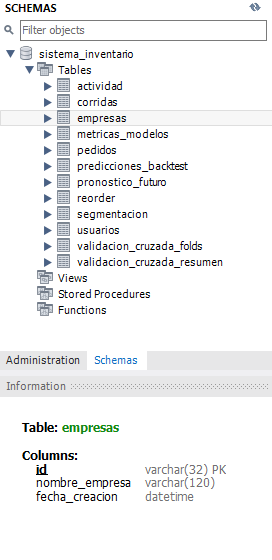
\includegraphics[height=0.35\textheight]{templatefigures/mysql_workbench_empresas}
    \caption{Estructura de la tabla \texttt{empresas} vista desde MySQL Workbench, conectado a la base de datos local.}
    \label{fig:mysql_workbench_empresas}
\end{figure}

La tabla \texttt{empresas} existe en la base de datos con las columnas descritas anteriormente: un identificador de tipo \texttt{varchar(32)} como clave primaria, el nombre de la empresa, y la fecha de creación del registro.

\begin{figure}[H]
    \centering
    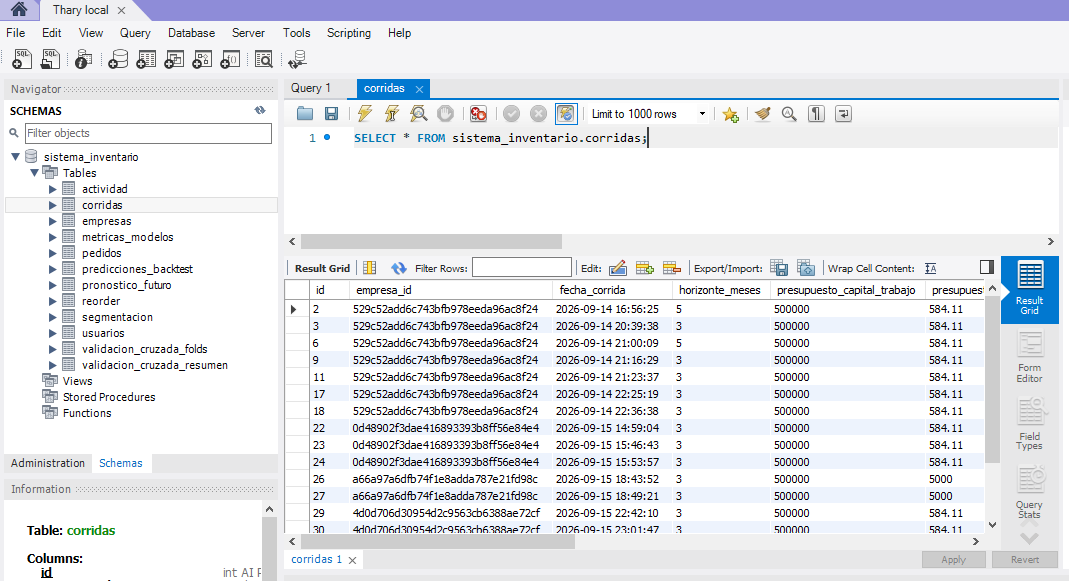
\includegraphics[height=0.3\textheight]{templatefigures/mysql_workbench_corridas}
    \caption{Consulta sobre la tabla \texttt{corridas} en MySQL Workbench, mostrando el esquema completo de 12 tablas y el historial acumulado de corridas.}
    \label{fig:mysql_workbench_corridas}
\end{figure}

La Fig. \ref{fig:mysql_workbench_corridas} muestra la confirmación de que cada procesamiento de archivo genera una fila nueva en \texttt{corridas} sin eliminar las anteriores. Existen múltiples filas asociadas a una misma empresa, correspondientes a distintas corridas realizadas en distintasfechas y horas.


\subsubsection{Diseño UX/UI}
% Guia: flujos de usuario, wireframes y criterios de usabilidad y accesibilidad.
El nombre del sistema "Thary" fue elegido en la etapa de diseño de identidad visual, es un nombre corto escogido por fonéticamente sonar similar a las últimas cuatro letras de la palabra "Inventory", (inventario en inglés). En cuanto a icono representativo, se eligió la figura de un buho, para transmitir la idea de orden y control, ya que los buhos son animales reconocidos por su capacidad de percepción y vigilancia, relacionado a como Thary se encarga de detectar señales de riesgo que podrían afectar el inventario de una empresa.

\begin{figure}[H]
    \centering
    
\includegraphics[width=0.5\textwidth]{templatefigures/logo}
    \caption{Logotipo de Thary, compuesto por el nombre del sistema y el icono representativo del búho}
    \label{fig:ux_login_logo}
\end{figure}

Para realizar el diseño de interacción de Thary, se decidió separar las pantallas en dos: Una dirigida exclusivamente a los administradores y otra dirigida a los empleados del inventario. Al ingresar al sistema, un usuario con el rol de administrador sigue el siguiente flujo:

El usuario inicia sesión o se registra de no tener una cuenta.

\begin{figure}[H]
    \centering
    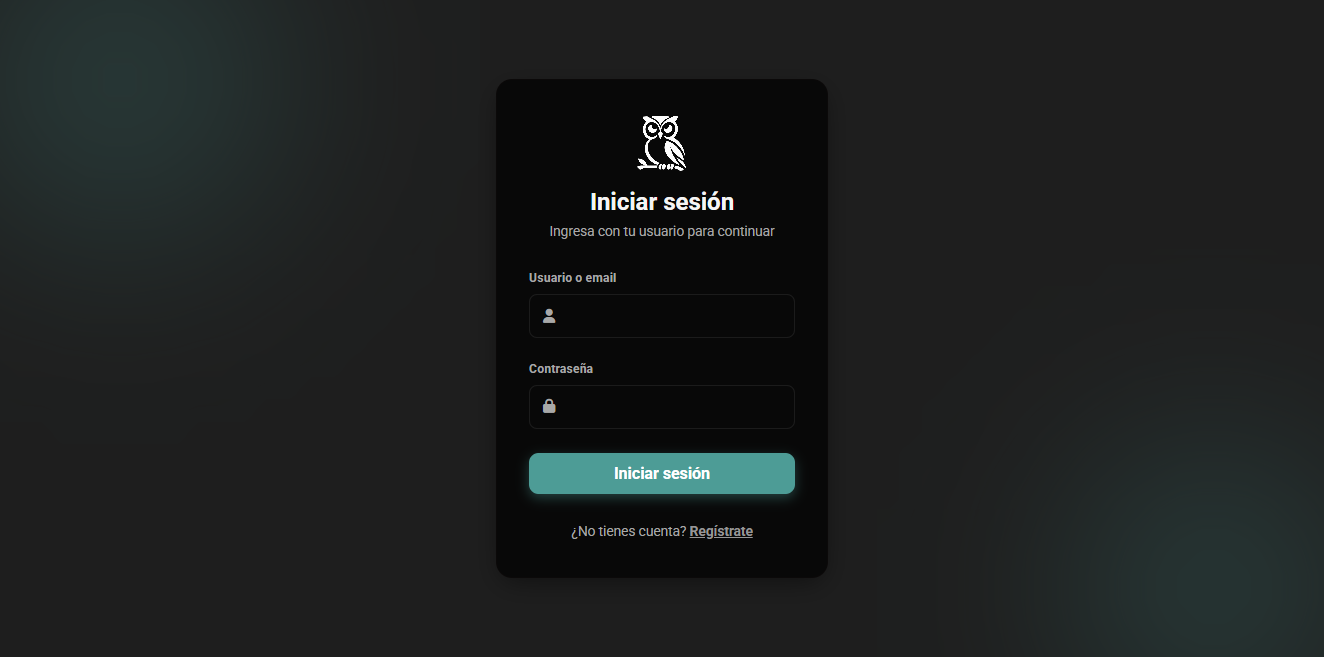
\includegraphics[width=0.5\textwidth]{templatefigures/ux_login}
    \caption{Pantalla de inicio de sesión de Thary}
    \label{fig:ux_login}
\end{figure}

\begin{figure}[H]
    \centering
    
\includegraphics[width=0.5\textwidth]{templatefigures/ux_registro}
    \caption{Pantalla de registro de Thary}
    \label{fig:ux_registro}
\end{figure}

El administrador inicia en la pantalla de inicio del sistema, desde la cual puede acceder a la funcionalidad de carga de archivo (\textit{index}), al haber cargado el archivo correctamente y que este sea válido, se le redirige automáticamente al dashboard, donde al seleccionar "Pronóstico de demanda", se muestran los resultados.

\begin{figure}[H]
    \centering
    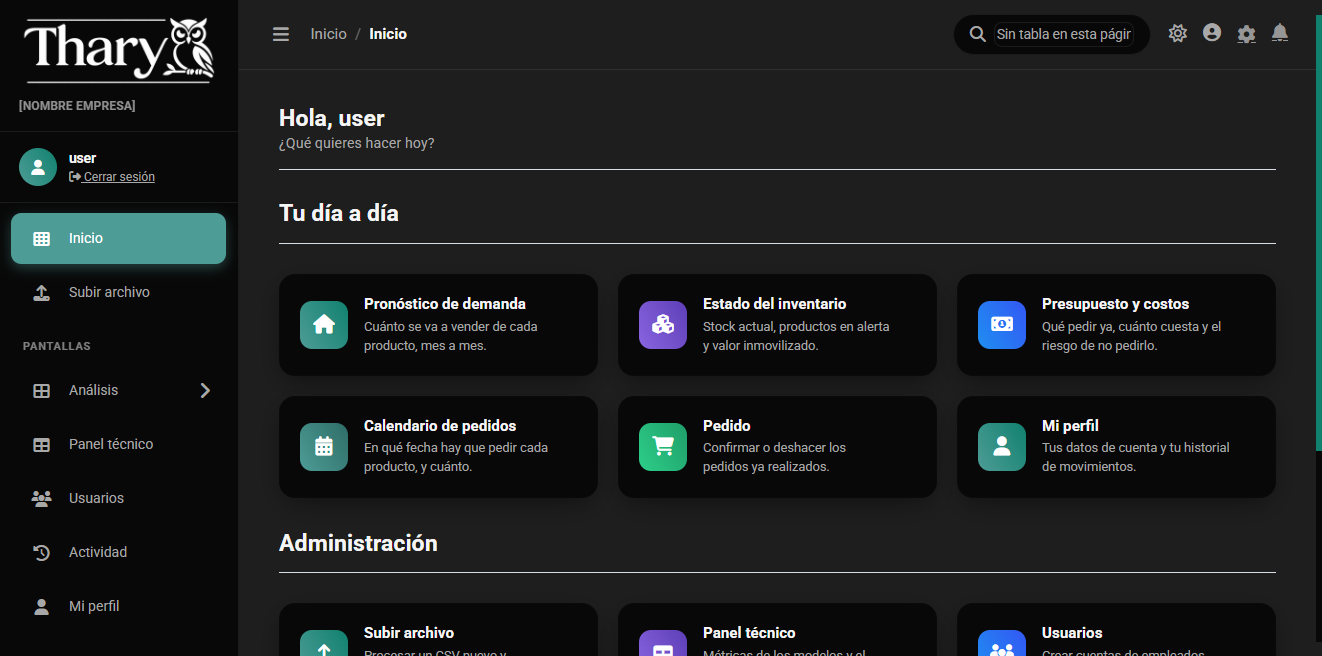
\includegraphics[width=0.5\textwidth]{templatefigures/ux_dashboard}
    \caption{Pantalla de dashboard de Thary}
    \label{fig:ux_dashboard}
\end{figure}


\begin{figure}[H]
    \centering
    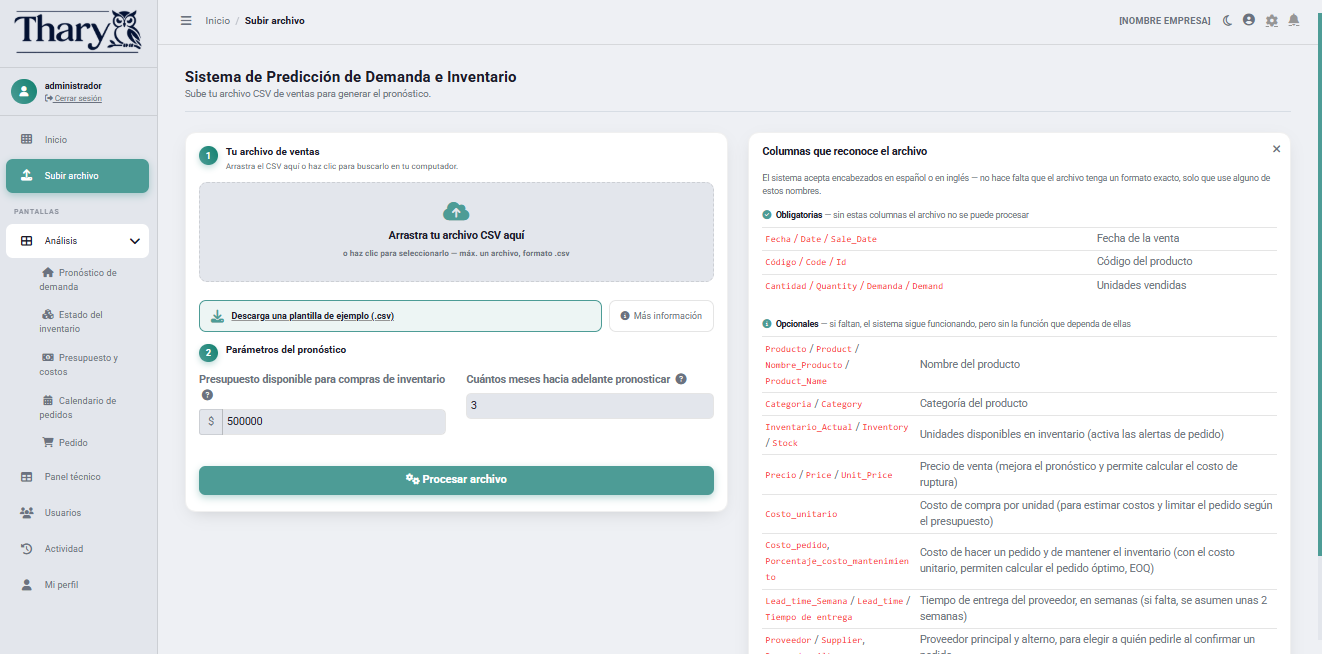
\includegraphics[width=0.5\textwidth]{templatefigures/ux_subir_archivo}
    \caption{Pantalla para subir archivos de Thary}
    \label{fig:ux_subir_archivo}
\end{figure}


\begin{figure}[H]
    \centering
    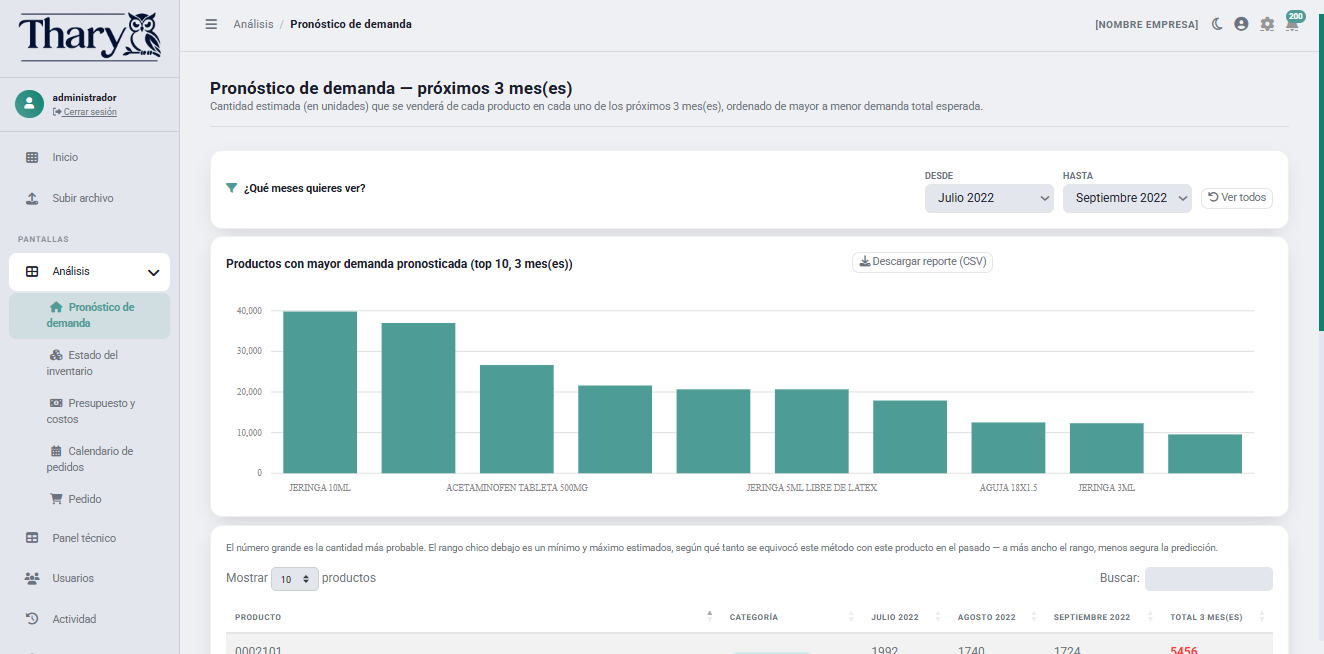
\includegraphics[width=0.5\textwidth]{templatefigures/ux_prediccion}
    \caption{Pantalla de predicción de demanda de Thary}
    \label{fig:ux_prediccion}
\end{figure}

En el sidebar, además de encontrar demas opciones como estado del inventario, presupuesto y pedidos, el administrador puede navegar hacia la gestión de usuarios, donde puede crear cuentas nuevas para su personal de inventario. 

\begin{figure}[H]
    \centering
    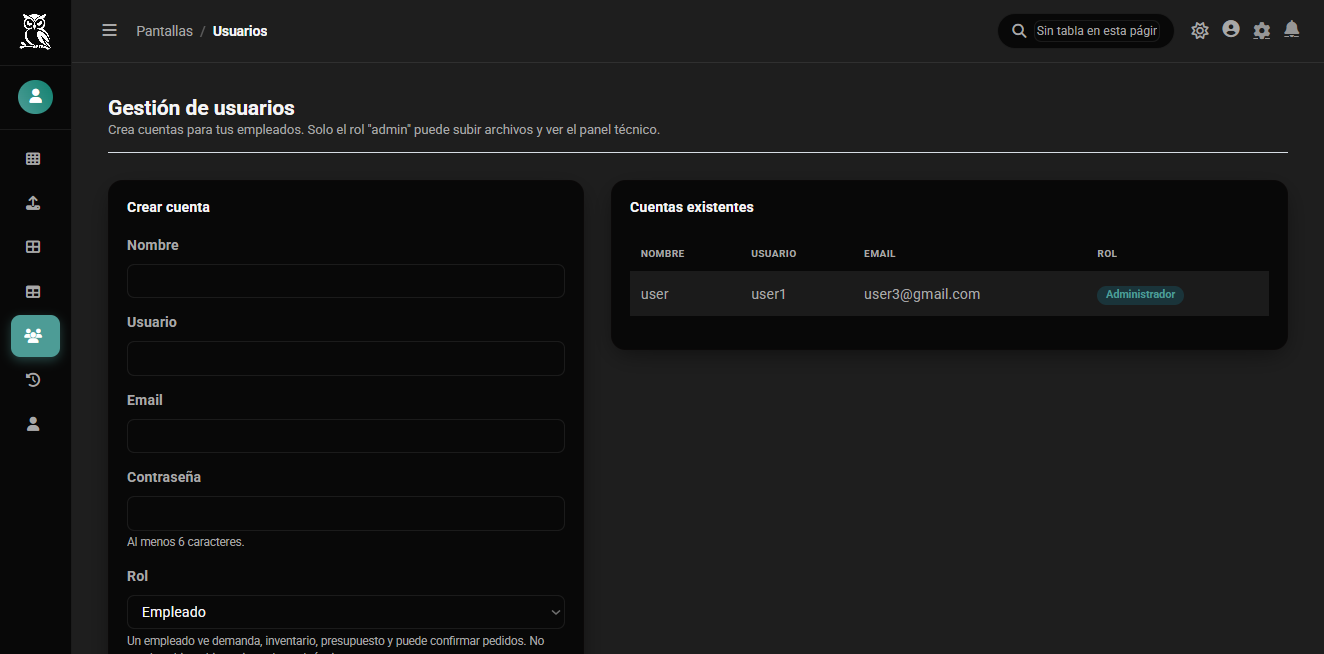
\includegraphics[width=0.5\textwidth]{templatefigures/ux_usuarios}
    \caption{Pantalla de gestión de usuarios de Thary}
    \label{fig:ux_usuarios}
\end{figure}

El flujo de los empleados es bastante similar, con la diferencia de que el perfil de un empleado cuenta con menos privilegios que el perfil de un administrador, por lo que al iniciar sesión, el empleado no puede subir ningún archivo,por lo que solo puede acceder al dashboard de la demanda pronosticada en base al csv que ya anteriormente fue cargado al sistema por el administrador que creó su cuenta, ya desde ahí, puede navegar a las mismas funcionalidades del análisis de los datos que el administrador: estado del inventario, presupuesto y pedidos. 

\begin{figure}[H]
    \centering
    \begin{subfigure}[b]{0.42\textwidth}
        \centering
        
\includegraphics[height=0.25\textheight]{templatefigures/ux_sidebar_empleado.png}
        \caption{Sidebar de empleado}
        \label{fig:ux_sidebar_empleado}
    \end{subfigure}
    \hspace{1cm}
    \begin{subfigure}[b]{0.42\textwidth}
        \centering
        
\includegraphics[height=0.25\textheight]{templatefigures/ux_sidebar_administrador.png}
        \caption{Sidebar de administrador}
        \label{fig:ux_sidebar_administrador}
    \end{subfigure}
\end{figure}

\begin{figure}[H]
    \centering
    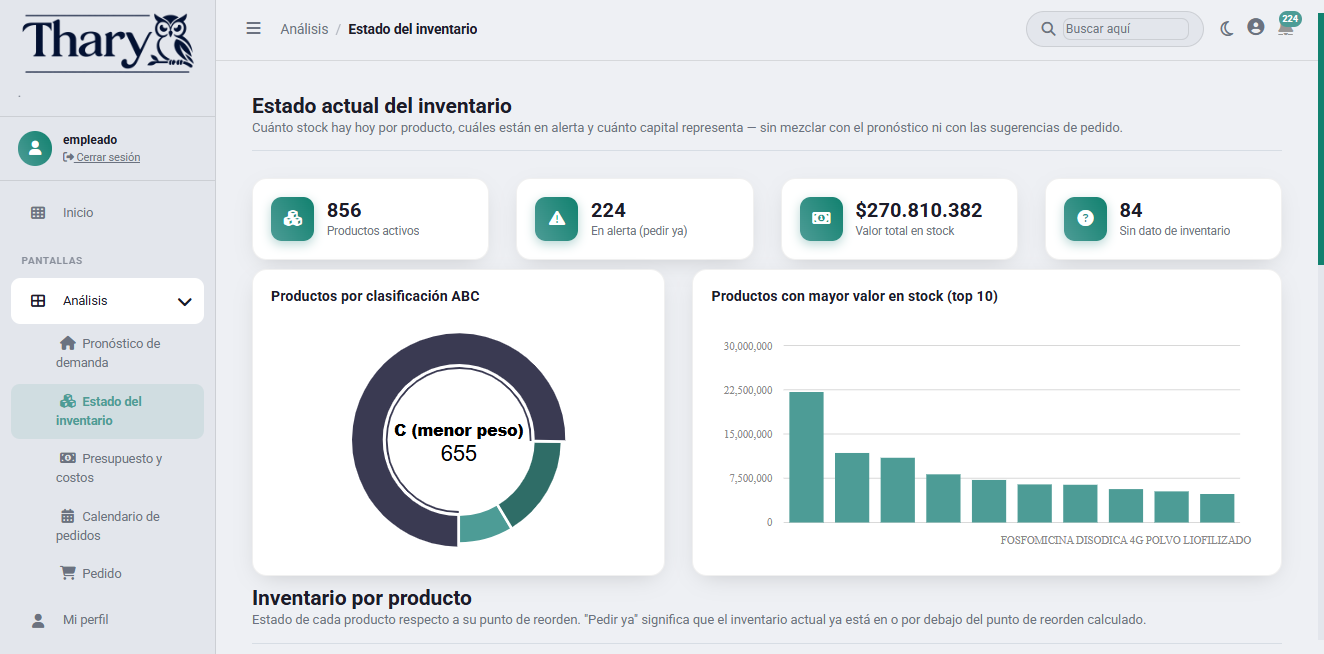
\includegraphics[height=0.25\textheight]{templatefigures/ux_estado_inventario.png}
    \caption{Estado del inventario}
    \label{fig:ux_estado_inventario}
\end{figure}

\begin{figure}[H]
    \centering
    \begin{subfigure}[b]{0.85\textwidth}
        \centering
        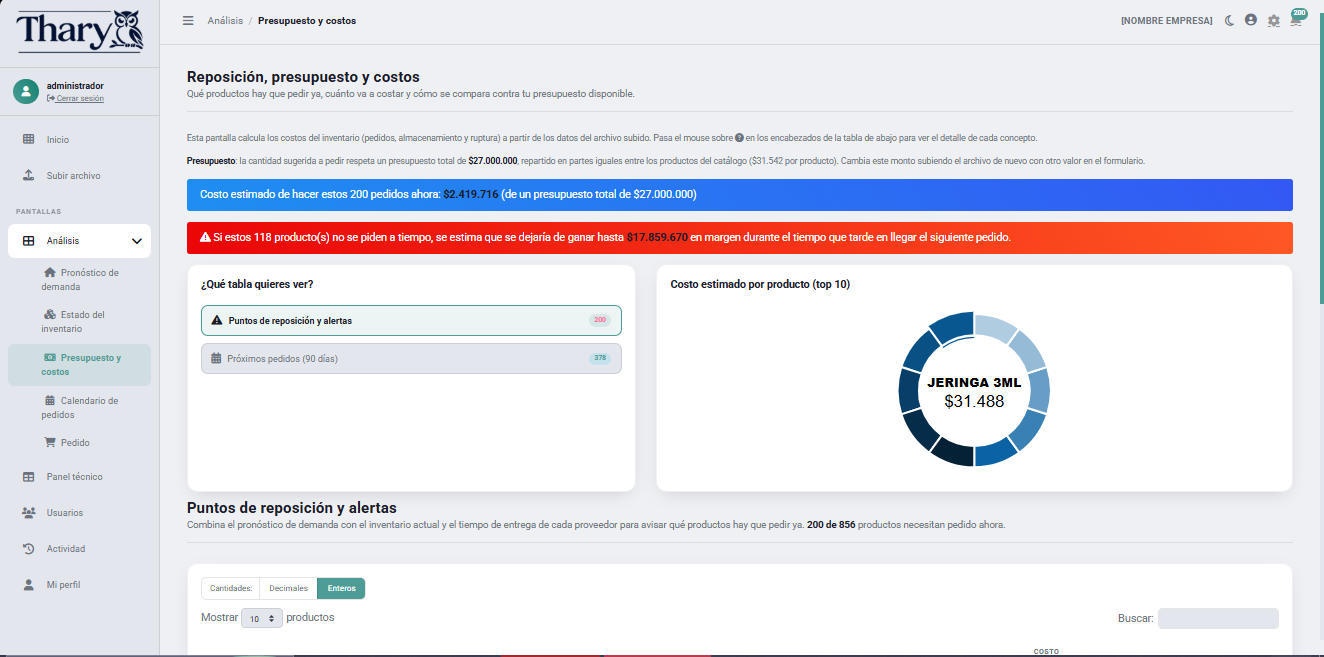
\includegraphics[width=\textwidth]{templatefigures/ux_presupuesto.png}
        \caption{Presupuesto}
        \label{fig:ux_presupuesto}
    \end{subfigure}

    \vspace{0.4cm}

    \begin{subfigure}[b]{0.85\textwidth}
        \centering
        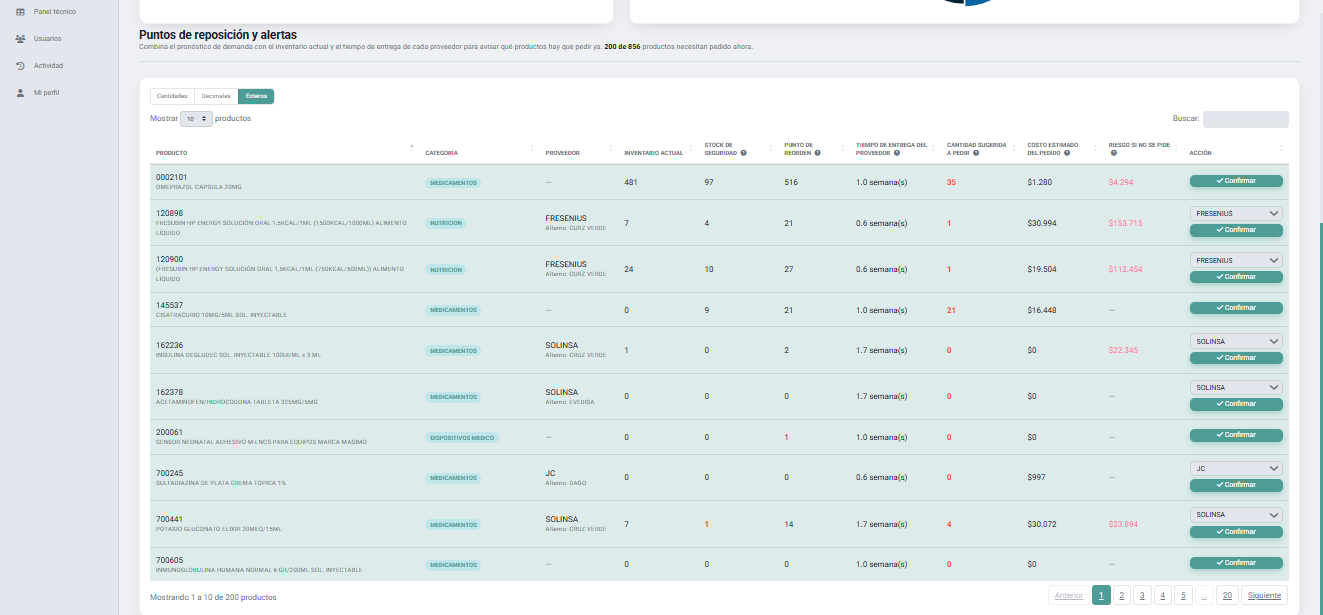
\includegraphics[width=\textwidth]{templatefigures/ux_reposicion_alertas.png}
        \caption{Alertas de reposición}
        \label{fig:ux_reposicion_alertas}
    \end{subfigure}
\end{figure}

La gestión de pedidos se puede ver en tres vistas: los pedidos sugeridos pendientes de confirmar, el historial de pedidos ya confirmados, y los próximos pedidos estimados según el calendario de reposición.

\begin{figure}[H]
    \centering
    \begin{subfigure}[b]{0.85\textwidth}
        \centering
        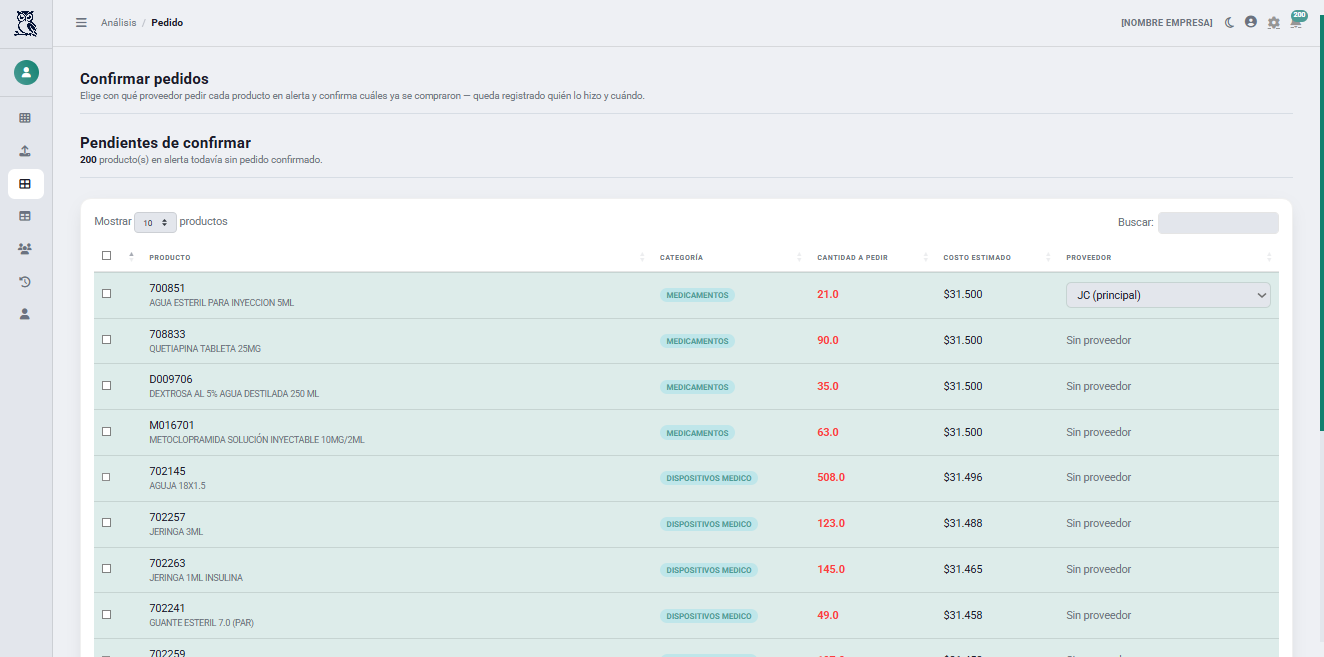
\includegraphics[width=\textwidth]{templatefigures/ux_pedidos.png}
        \caption{Lista de Pedidos}
        \label{fig:ux_pedidos}
    \end{subfigure}

    \vspace{0.4cm}

    \begin{subfigure}[b]{0.85\textwidth}
        \centering
        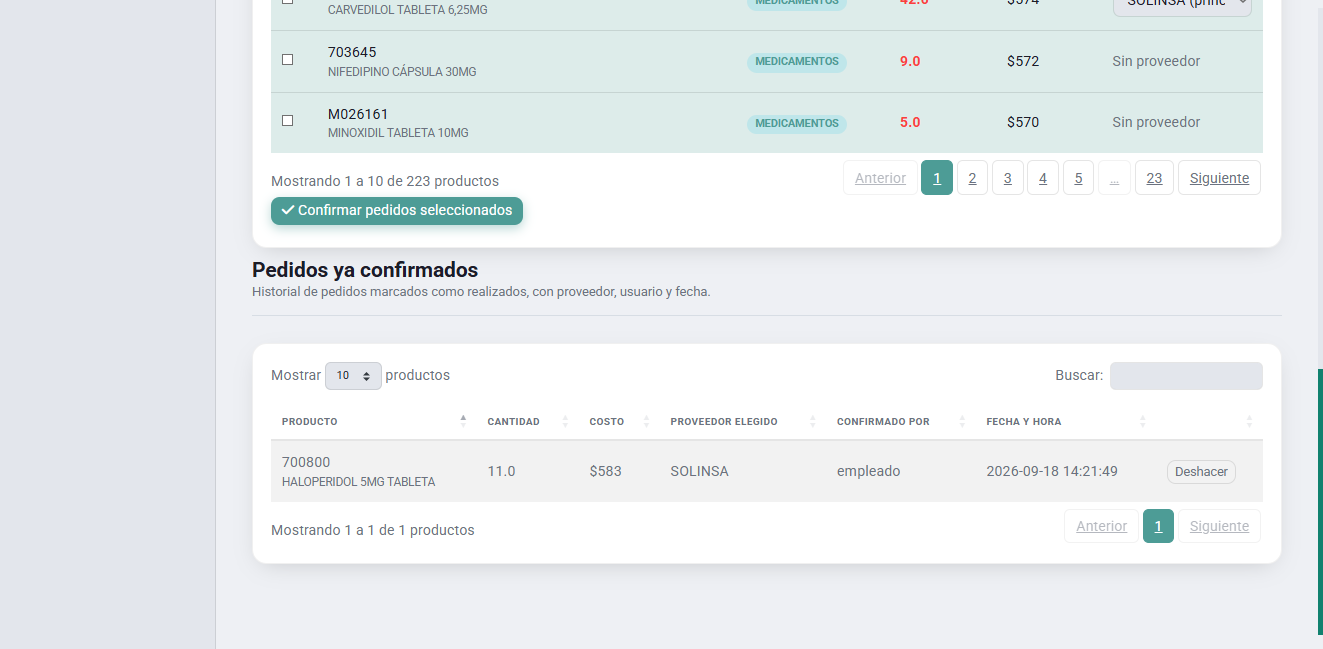
\includegraphics[width=\textwidth]{templatefigures/ux_pedidos_confirmados.png}
        \caption{Pedidos confirmados}
        \label{fig:ux_pedidos_confirmados}
    \end{subfigure}
\end{figure}

\begin{figure}[H]
    \centering
    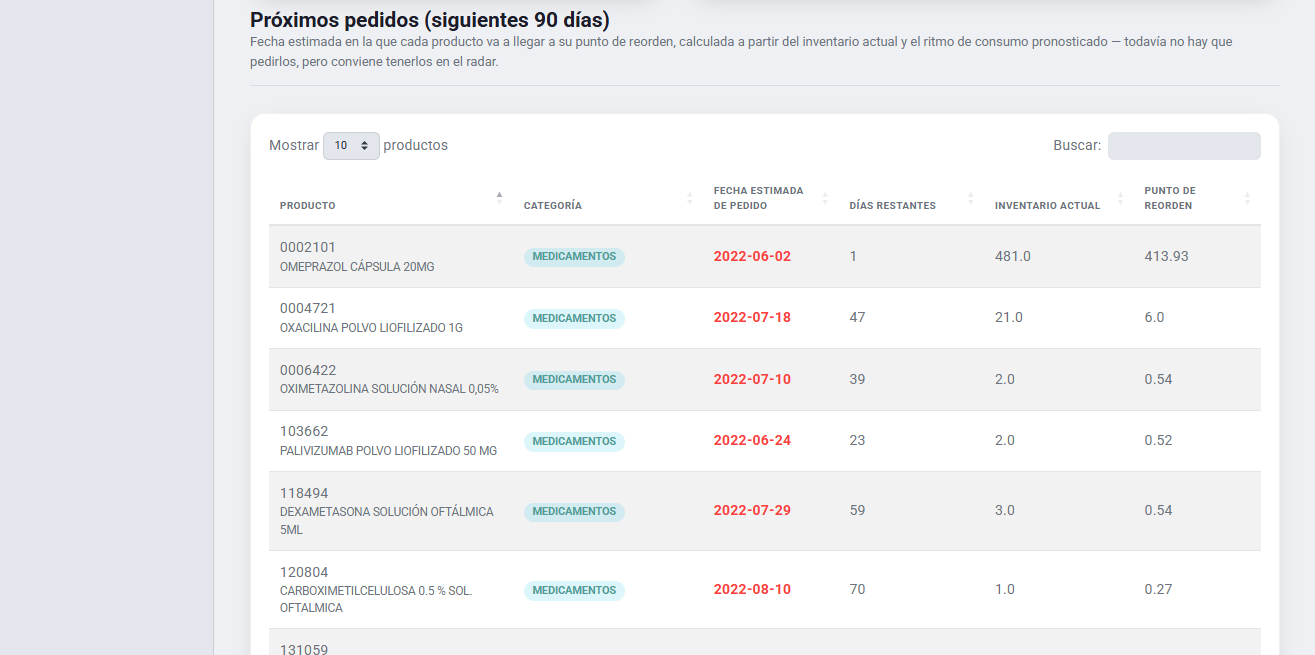
\includegraphics[height=0.25\textheight]{templatefigures/ux_prox_pedidos.png}
    \caption{Próximos pedidos}
    \label{fig:ux_prox_pedidos}
\end{figure}

\begin{figure}[H]
    \centering
    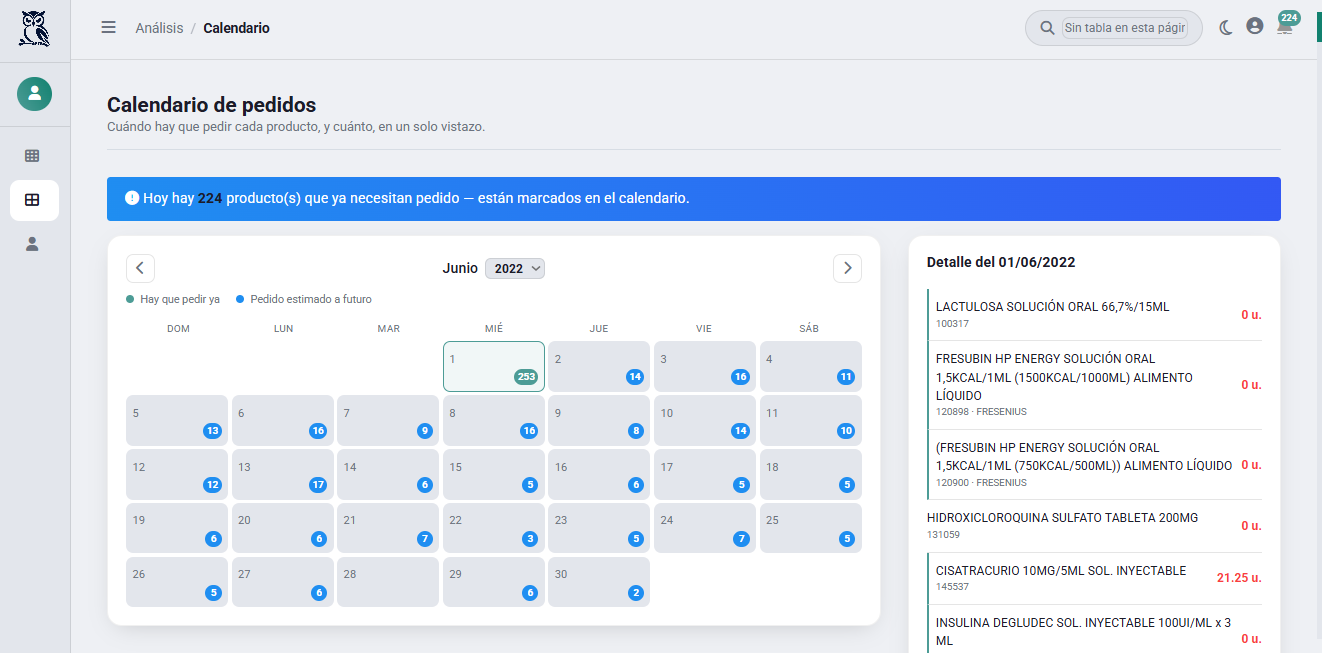
\includegraphics[height=0.25\textheight]{templatefigures/ux_calendario_pedidos.png}
    \caption{Calendario de pedidos}
    \label{fig:ux_calendario_pedidos}
\end{figure}

Una vez finalizadas sus tareas, los usuarios pueden cerrar sesión en su cuenta.

\begin{figure}[H]
    \centering
    
\includegraphics[width=0.5\textwidth]{templatefigures/ux_cerrar_sesion.png}
    \caption{Cerrar sesión}
    \label{fig:ux_cerrar_sesion}
\end{figure}

Los criterios de usabilidad que fueron tomados en cuenta fueron:

\begin{itemize}
    \item Uso de alertas visuales codificadas por color para indicar fácilmente que productos se encuentran en o por debajo de su punto de reposición y requieren ser reabastecidos inmediatamente.
    
    \begin{figure}[H]
    \centering
    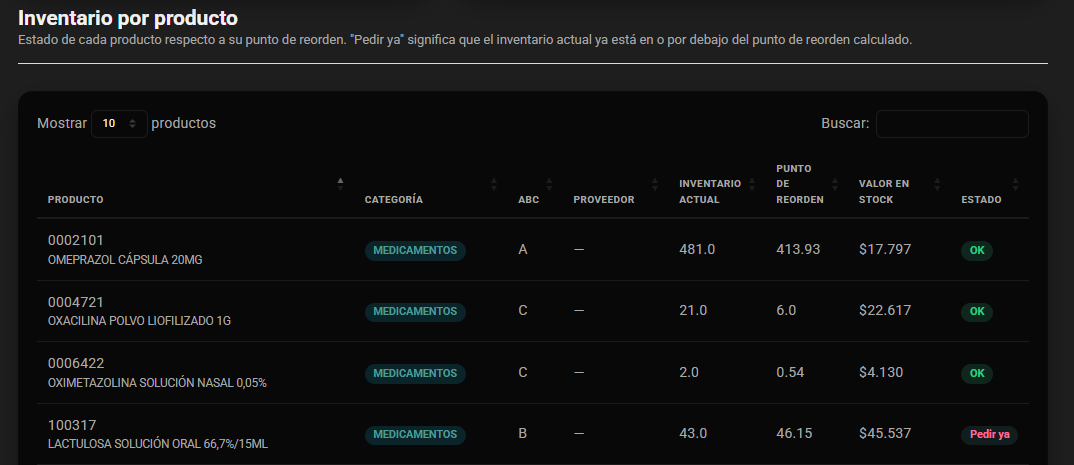
\includegraphics[width=0.5\textwidth]{templatefigures/ux_alertas_visuales.png}
    \caption{Alertas visuales}
    \label{fig:ux_alertas_visuales}
    \end{figure}

    \item Cuando un usuario con el rol de empleado inicie sesión, pero su respectivo administrador no subió ningún archivo csv, en vez de ver la pantalla del dashboard, verá una pantalla con el mensaje de que una vez el admin cargue el archivo, podrá ver los análisis.

    \begin{figure}[H]
    \centering
    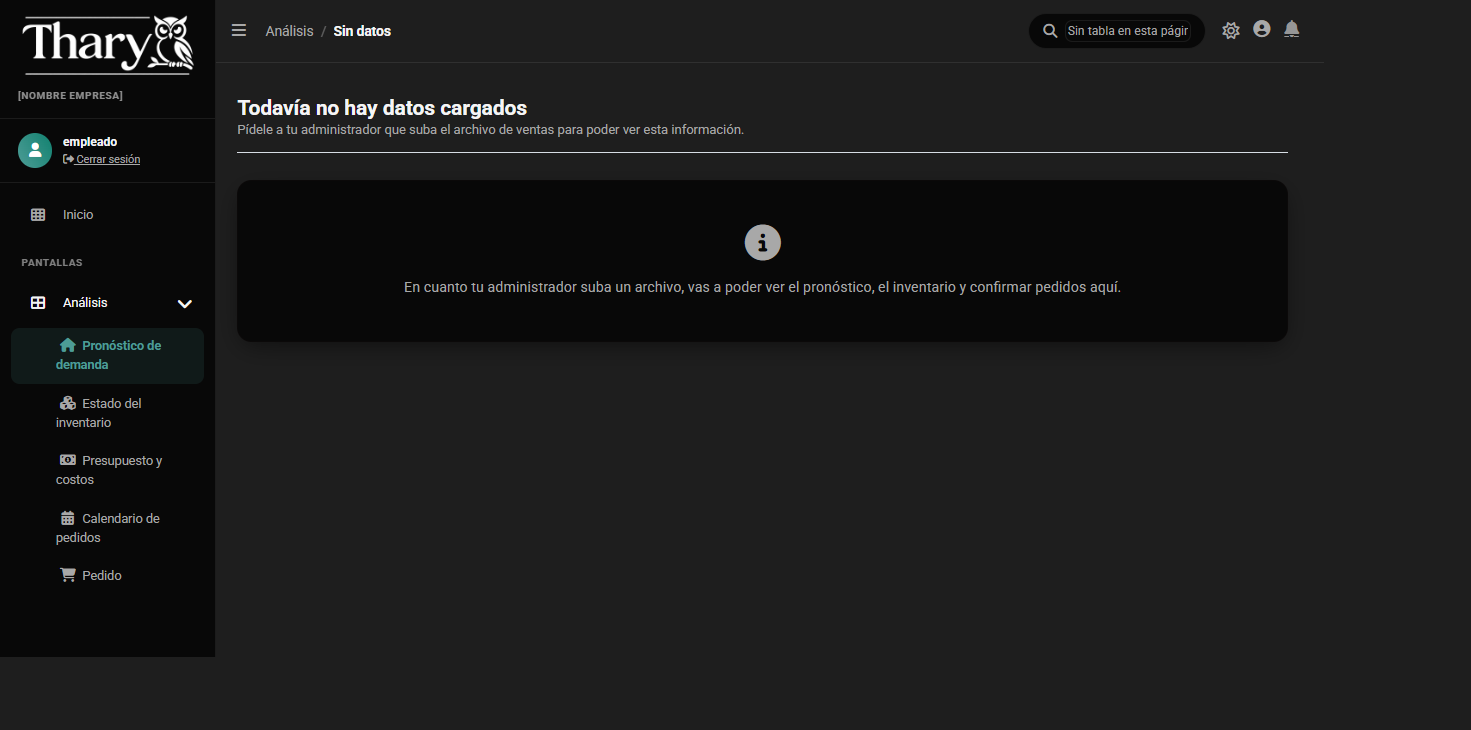
\includegraphics[width=0.5\textwidth]{templatefigures/ux_dashboard_empleado.png}
    \caption{Dashboard del empleado}
    \label{fig:ux_dashboard_empleado}
    \end{figure}
    
    \item El sistema cuenta con un modo oscuro y modo claro para que el usuario pueda escoger según sus preferencias, mejorando la usabilidad ofreciendo ventajas como comodidad visual, menor fatiga en uso prolongado, contraste, etc.

    \begin{figure}[H]
    \centering
    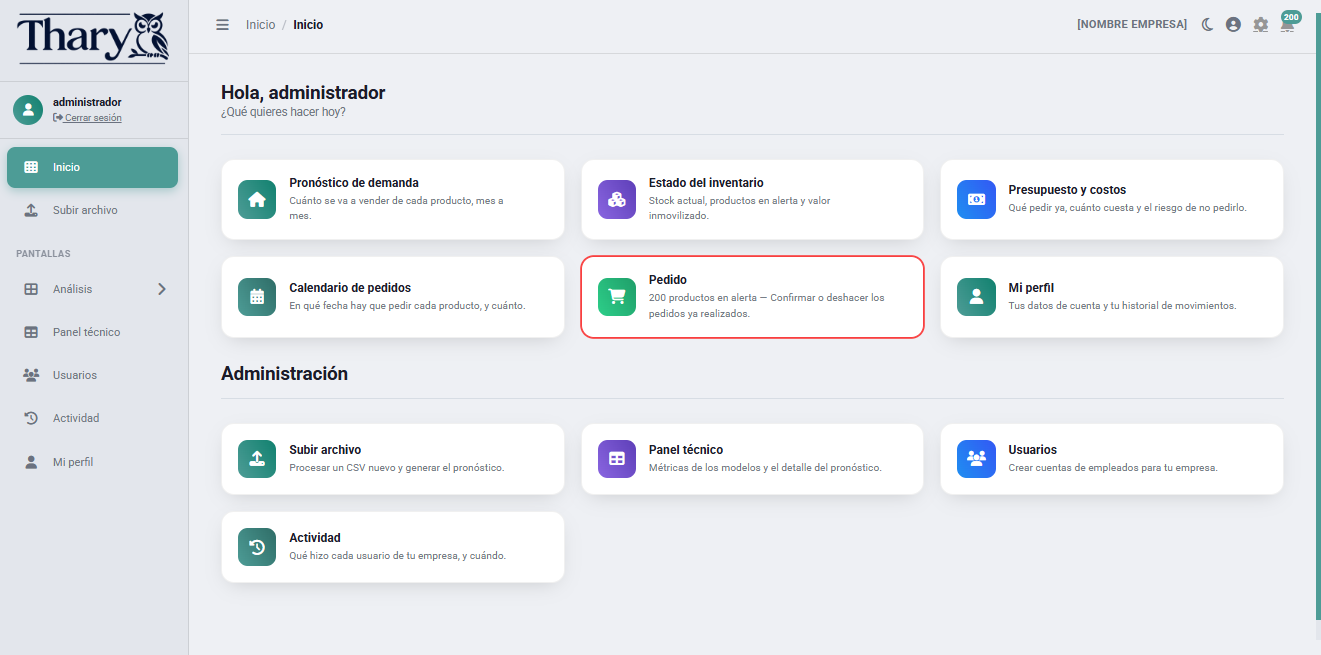
\includegraphics[width=0.5\textwidth]{templatefigures/ux_dashboard_claro.png}
    \caption{Dashboard en modo claro}
    \label{fig:ux_dashboard_claro}
    \end{figure}

    \item Thary cuenta con una versión mobile, la cual le permite al usuario poder acceder a todas las funcionalidades de la versión de escritorio desde su teléfono móvil.

        \begin{figure}[H]
    \centering
    
\includegraphics[width=0.5\textwidth]{templatefigures/ux_dashboard_mobile.png}
    \caption{Dashboard en modo mobile}
    \label{fig:ux_dashboard_mobile}
    \end{figure}
\end{itemize}

En cuanto a criterios de accesibilidad, se tomaron en cuenta los criterios de usabilidad, pero no se tomaron en cuenta mecanismos adicionales para hacer más accesible el sistema como algún tipo de lector de pantalla para personas con discapacidad visual, o implementar un sistema de navegación completa por teclado para alguna persona que no pueda usar un mouse. Estas falencias se reconocen como una limitación del diseño actual, y se espera mejorarlas en el futuro. 
